% LaTeX Template For MATH 490 @ VCU
\documentclass[11pt]{book}

\linespread{2}
\setlength{\textwidth}{6.9in}
\setlength{\textheight}{8.5in}
\setlength{\oddsidemargin}{-0.2in}
\setlength{\evensidemargin}{-0.2in}
\setlength{\topmargin}{-0.1in}
\setlength{\headheight}{0.1in}
\setlength{\headsep}{0.4in}
\setlength{\footskip}{0.4in}
\setlength{\delimitershortfall}{13.5pt}
\delimiterfactor=100

\usepackage{hyperref}
\usepackage{amsmath}
\usepackage{amsthm}
\usepackage{amssymb}
\usepackage{enumerate}
\usepackage{enumitem}
\usepackage{titlesec}
\usepackage{multicol}
\usepackage{multirow}
\usepackage{mathtools}
\usepackage{mdframed}
\usepackage{tocloft}
\usepackage{tcolorbox}
\usepackage{extarrows}
\usepackage{libertine}
\usepackage[libertine]{newtxmath}

\setlist{nosep}
\setlist[enumerate]{label=\roman*.}

\setlength{\multicolsep}{6.2pt}

\renewcommand{\arraystretch}{0.85}

\definecolor{defcolor}{RGB}{255,236,236}    % light red
\definecolor{ngtcolor}{RGB}{255,242,242}    % lighter red
\definecolor{lnkcolor}{RGB}{0,0,180}        % blue
\definecolor{thmcolor}{RGB}{236,236,255}    % light blue
\definecolor{lemcolor}{RGB}{239,239,255}    % lighter blue
\definecolor{procolor}{RGB}{242,242,255}    % lighter lighter blue
\definecolor{crlcolor}{RGB}{245,245,255}    % lighter lighter lighter blue
\definecolor{xmpcolor}{RGB}{255,240,225}    % light orange
\definecolor{rmkcolor}{RGB}{233,255,235}    % light green
\definecolor{axicolor}{RGB}{255,255,233}    % light yellow
\definecolor{notcolor}{RGB}{255,255,244}    % lighter yellow
\definecolor{whacolor}{RGB}{250,250,250}    % lighter gray
\definecolor{reccolor}{RGB}{255,244,255}    % lighter purple

\hypersetup{
    colorlinks,
    citecolor=lnkcolor,
    filecolor=lnkcolor,
    linkcolor=lnkcolor,
    urlcolor=lnkcolor
}

\newtheoremstyle{break}
    {\topsep/1.5} % space above
    {\topsep/1.5} % space below
    {}          % body font
    {}          % indent amount
    {\rmfamily} % theorem head font
    {.}          % punctuation after theorem head
    {0.5em}  % space after theorem head
    {\textbf{\thmname{#1}\thmnumber{ #2}}\thmnote{\text{ (#3)}}}
                % theorem hed spec. (empty = "normal")

\newtheoremstyle{no_label}
    {\topsep/1.5} % space above
    {\topsep/1.5} % space below
    {}          % body font
    {}          % indent amount
    {\rmfamily} % theorem head font
    {.}          % punctuation after theorem head
    {0.5em}  % space after theorem head
    {\textbf{\thmname{#1}\thmnumber{}}\thmnote{\text{ (#3)}}}
                % theorem hed spec. (empty = "normal")

\theoremstyle{break}
\newmdtheoremenv[
    backgroundcolor=thmcolor,
    linecolor=black,
    linewidth=1pt,
    topline=true,
    bottomline=true,
    rightline=true,
    skipabove=\topsep/1.5,
    skipbelow=\topsep/1.5
]{theorem}{Theorem}[section]
\newmdtheoremenv[
    backgroundcolor=crlcolor,
    linecolor=black,
    linewidth=1pt,
    topline=true,
    bottomline=true,
    rightline=true,
    skipabove=\topsep/1.5,
    skipbelow=\topsep/1.5
]{corollary}[theorem]{Corollary}
\newmdtheoremenv[
    backgroundcolor=lemcolor,
    linecolor=black,
    linewidth=1pt,
    topline=true,
    bottomline=true,
    rightline=true,
    skipabove=\topsep/1.5,
    skipbelow=\topsep/1.5
]{lemma}[theorem]{Lemma}
\newmdtheoremenv[
    backgroundcolor=axicolor,
    linecolor=black,
    linewidth=1pt,
    topline=true,
    bottomline=true,
    rightline=true,
    skipabove=\topsep/1.5,
    skipbelow=\topsep/1.5
]{axiom}[theorem]{Axiom}
\newmdtheoremenv[
    backgroundcolor=procolor,
    linecolor=black,
    linewidth=1pt,
    topline=true,
    bottomline=true,
    rightline=true,
    skipabove=\topsep/1.5,
    skipbelow=\topsep/1.5
]{proposition}[theorem]{Proposition}
\newmdtheoremenv[
    backgroundcolor=defcolor,
    linecolor=black,
    linewidth=1pt,
    topline=true,
    bottomline=true,
    rightline=true,
    skipabove=\topsep/1.5,
    skipbelow=\topsep/1.5
]{definition}[theorem]{Definition}
\newmdtheoremenv[
    backgroundcolor=whacolor,
    linecolor=black,
    linewidth=1pt,
    topline=true,
    bottomline=true,
    rightline=true,
    skipabove=\topsep/1.5,
    skipbelow=\topsep/1.5
]{problem}[theorem]{Problem}
\newmdtheoremenv[
    backgroundcolor=whacolor,
    linecolor=black,
    linewidth=1pt,
    topline=true,
    bottomline=true,
    rightline=true,
    skipabove=\topsep/1.5,
    skipbelow=\topsep/1.5
]{exercise}[theorem]{Exercise}

\theoremstyle{no_label}
\newmdtheoremenv[
    backgroundcolor=whacolor,
    linecolor=black,
    linewidth=1pt,
    topline=true,
    bottomline=true,
    rightline=true,
    skipabove=\topsep/1.5,
    skipbelow=\topsep/1.5
]{question}{Question}
\newmdtheoremenv[
    backgroundcolor=reccolor,
    linecolor=black,
    linewidth=1pt,
    topline=true,
    bottomline=true,
    rightline=true,
    skipabove=\topsep/1.5,
    skipbelow=\topsep/1.5
]{recall}{Recall}
\newmdtheoremenv[
    backgroundcolor=notcolor,
    linecolor=black,
    linewidth=1pt,
    topline=true,
    bottomline=true,
    rightline=true,
    skipabove=\topsep/1.5,
    skipbelow=\topsep/1.5
]{notation}{Notation}
\newmdtheoremenv[
    backgroundcolor=rmkcolor,
    linecolor=black,
    linewidth=1pt,
    topline=true,
    bottomline=true,
    rightline=true,
    skipabove=\topsep/1.5,
    skipbelow=\topsep/1.5
]{remark}{Remark}
\newmdtheoremenv[
    backgroundcolor=xmpcolor,
    linecolor=black,
    linewidth=1pt,
    topline=true,
    bottomline=true,
    rightline=true,
    skipabove=\topsep/1.5,
    skipbelow=\topsep/1.5
]{example}{Example}

\DeclareMathOperator{\arcsec}{arcsec}
\DeclareMathOperator{\arccot}{arccot}
\DeclareMathOperator{\arccsc}{arccsc}
\DeclareMathOperator{\interior}{int}
\DeclareMathOperator{\closure}{cl}
\DeclareMathOperator{\boundary}{bd}

\newcommand{\derivative}{D\!\,}
\newcommand{\scndderivative}{D^2\!\,}
\newcommand{\diff}[2]{\dfrac{\dd{#1}}{\dd{#2}}}
\newcommand{\dirderivative}[1]{D_{#1}\:}
\newcommand{\pderivative}[2]{\dfrac{\partial {#1}}{\partial {#2}}}
\newcommand{\scndpderivative}[3]{\dfrac{\partial^2 {#1}}{\partial {#3}\partial {#2}}}
\newcommand{\dd}{\text{d}}
\newcommand{\ddi}{\text{$\,$d}}
\newcommand{\qqed}{{\hfill$\blacksquare$}}
\newcommand{\defeq}{\overset{\text{def}}{=}}
\newcommand{\transpose}{\text{T}}
\newcommand{\bbR}{\mathbb{R}}
\newcommand{\bbN}{\mathbb{N}}
\newcommand{\calL}{\mathcal{L}}
\newcommand{\bfzero}{\textbf{0}}
\newcommand{\bfa}{\textbf{a}}
\newcommand{\bfb}{\textbf{b}}
\newcommand{\bfe}{\textbf{e}}
\newcommand{\bff}{\textbf{f}}
\newcommand{\bfg}{\textbf{g}}
\newcommand{\bfh}{\textbf{h}}
\newcommand{\bfr}{\textbf{r}}
\newcommand{\bfv}{\textbf{v}}
\newcommand{\bfu}{\textbf{u}}
\newcommand{\bfx}{\textbf{x}}
\newcommand{\bfy}{\textbf{y}}
\newcommand{\bfalpha}{\text{\boldmath$\alpha$}}
\newcommand{\bfepsilon}{\text{\boldmath$\epsilon$}}
\newcommand{\bfvarepsilon}{\text{\boldmath$\varepsilon$}}
\newcommand{\figtag}[1]{\\[-1.2em]Figure {#1}}
\newcommand{\pfexercise}{This is an exercise left to the reader.}

\setcounter{section}{0}
\numberwithin{equation}{section}

\makeatletter
\newcommand{\vast}{\bBigg@{4}}
\newcommand{\Vast}{\bBigg@{5}}
\g@addto@macro\normalsize{
    \setlength\abovedisplayskip{0em}
    \setlength\belowdisplayskip{0em}
}
\makeatother

\newcommand*\samethanks[1][\value{footnote}]{\footnotemark[#1]}

\title{\textbf{Introduction to Differential and Integral Calculus}}
\author{Chang, Yung-Hsuan}

\begin{document}
\maketitle
\thispagestyle{empty}
\newpage
\pagenumbering{roman}
\newpage
\phantomsection
\addcontentsline{toc}{chapter}{Contents}
\tableofcontents
\newpage

\phantomsection
\addcontentsline{toc}{chapter}{Preface}
\chapter*{Preface}

This book is summarized by Yung-Hsuan Chang refering to \emph{Calculus: One and Several Variables}, 10th edition and \emph{Calculus: Early Treanscendentals}, 9th edition.

\newpage
\pagenumbering{arabic}

\chapter{Review of Elementary Mathematics}

To a Roman in the days of the empire, a “calculus” was a pebble used in counting and gambling. Centuries later, “calculare” came to mean “to calculate,” “to compute,” “to figure out.” For our purposes, calculus is elementary mathematics (algebra, geometry, trigonometry) enhanced by the limit process.

Generally speaking, calculus takes ideas from elementary mathematics and extends them to a more general situation: 
\begin{enumerate}
    \item from tangent line to a straight line to one to a curve,
    \item from area of a polygon to are of a region bounded by curves,
    \item from volume of a rectangular solid to volume of a solid with a curved boundary, etc.
\end{enumerate}

\section{Basics}

In this section we review the terminology, notation, and formulas of elementary mathematics.

\subsection*{Sets}

\begin{definition}[Set]
    A \underline{set} is a collection of objects. We call objects in a set \underline{elements} or \underline{members} of the set. A set is usually denoted with a capital letter.
\end{definition}

For a collection of objects to be a set it must be well-defined; that is, given any object $x$, it must be possible to determine with certainty whether or not $x$ is an element of the set. Thus, the collection of all even numbers, the collection of all lines parallel to a given line $L$, and the solutions of the equation $$x^2 = 9$$ are all sets. The collection of all intelligent adults is not a set. It's not clear who should be included.

\begin{notation}
    We have some common symbols for you as statements:
    \begin{center}
        \begin{tabular}{rcl}
            $x\in A$ && the object $x$ is in the set $A$\\
            $x\notin A$ && the object $x$ is not in the set $A$\\
            $A\subseteq B$ && the set $A$ is a subset of the set $B$, i.e., any element in $A$ is in $B$\\
            $A\supseteq B$ && the set $A$ contains the set $B$, i.e., $B$ is a subset of $A$\\
            $A=B$ && the set $A$ equals the set $B$, i.e., both $A\subseteq B$ and $B\subseteq A$ hold
        \end{tabular}
    \end{center}
    We have some more symbols as operations:
    \begin{center}
        \begin{tabular}{rcl}
            $A\cup B$ && the union of set $A$ and set $B$\\
            $A\cap B$ && the intersection of set $A$ and set $B$\\
            $A^c$ && the complement of set $A$, i.e., the collection of all objects that is not in $A$\\
            $A\setminus B$ && the difference of set $A$ and set $B$, i.e., $A\cap B^c$\\
            $\emptyset$ && the set with no elements
        \end{tabular}
    \end{center}
\end{notation}

One can define a set with several ways:
\begin{itemize}
    \item roster, listing its elements between curly brackets, separated by commas, e.g, $$A=\{42, 520\}, \qquad B=\{e, \sqrt{2}, \pi\};$$
    \item semantic, using a rule to determine what the elements are, e.g, $$\text{Let $C$ be the set whose members are the first four positive integers;}$$
    \item set-builder, specifying a set as a selection from a larger set, determined by a condition on the elements, e.g., $$D=\{n\in\bbN\mid 0\leq n\leq 59\}.$$
\end{itemize}

We will have some examples for you as a reference. Of course, we will have exercises.

\subsection*{The Real Number System}

We start to learn counting from the set of all natural numbers (positive integers) $$\bbN=\{1, 2, 3, 4, 5, \dots\}.$$ After we graduated the elementary school, we obtained the expended concept of the set of integers $$\mathbb{Z}=\{0, 1, -1, 2, -2, \dots\}=\{a - b\mid a\in\bbN\text{\ and \ }b\in\bbN\},$$ the set of ratial numbers $$\mathbb{Q}=\{a/b\mid a\in\mathbb{Z}\text{\ and\ }b\in\bbN\},$$ and the set of real numbers $\bbR$. The construction (definition) of $\bbR$ is quite tedious. A relatively formal way to define $\bbR$ is to define $\bbR$ as the unique set contains $\mathbb{Q}$ with the least upper bound property. Since it is out of the scope of this book, we skip more definitions. One can imagine that $\bbR$ is the collection of all non-complex numbers that you have learned so far. These sets are so crucial that mathematicians use special letters $\mathbb{N}, \mathbb{Z}, \mathbb{Q}, \bbR$ to indicate such.

\begin{corollary}
    From the texts above, the containing relation $$\bbN\subseteq\mathbb{Z}\subseteq\mathbb{Q}\subseteq\bbR$$ holds.
\end{corollary}

\begin{proposition} The real number system $\bbR$ and the rationals $\mathbb{Q}$ are closed under addition and multiplication. That is, the product and the sum of two real (rational, respectively) numbers must be real (rational).
\end{proposition}

\begin{proposition}
    The real number system $\bbR$ and the rationals $\mathbb{Q}$ are dense. That is, there must be a real (rational, respectively) between two real numbers (rational numbers).
\end{proposition}

\subsection*{Order Properties}

In the real number system, we have the so-called order properties. 

\begin{theorem}[Order in the Real Number System]
    Let $a, b, c\in\bbR$. The following statements always hold.
    \begin{enumerate}
        \item (\textit{Trichotomy}) Either $a<b$, $a>b$, or $a=b$.
        \item (\textit{Transitivity}) If $a<b$ and $b<c$, then $a<c$.
        \item If $a<b$, then $a+r<b+r$ for all $r\in\bbR$.
        \item If $a<b$ and $c>0$, then $ac>bc$.
        \item If $a<b$ and $c<0$, then $ac<bc$.
    \end{enumerate}
\end{theorem}

\subsection*{The Number Line}

On a horizontal line we choose a point $O$. We call this point the origin and assign to it coordinate $0$. Now we choose a point $U$ to the right of $O$ and assign to it coordinate $1$. See Figure 1.1.1. The distance between $O$ and $U$ determines a scale (a unit length). We go on as follows: the point a units to the right of $O$ is assigned coordinate $a$; the point a units to the left of $O$ is assigned coordinate $-a$.

\begin{center}
    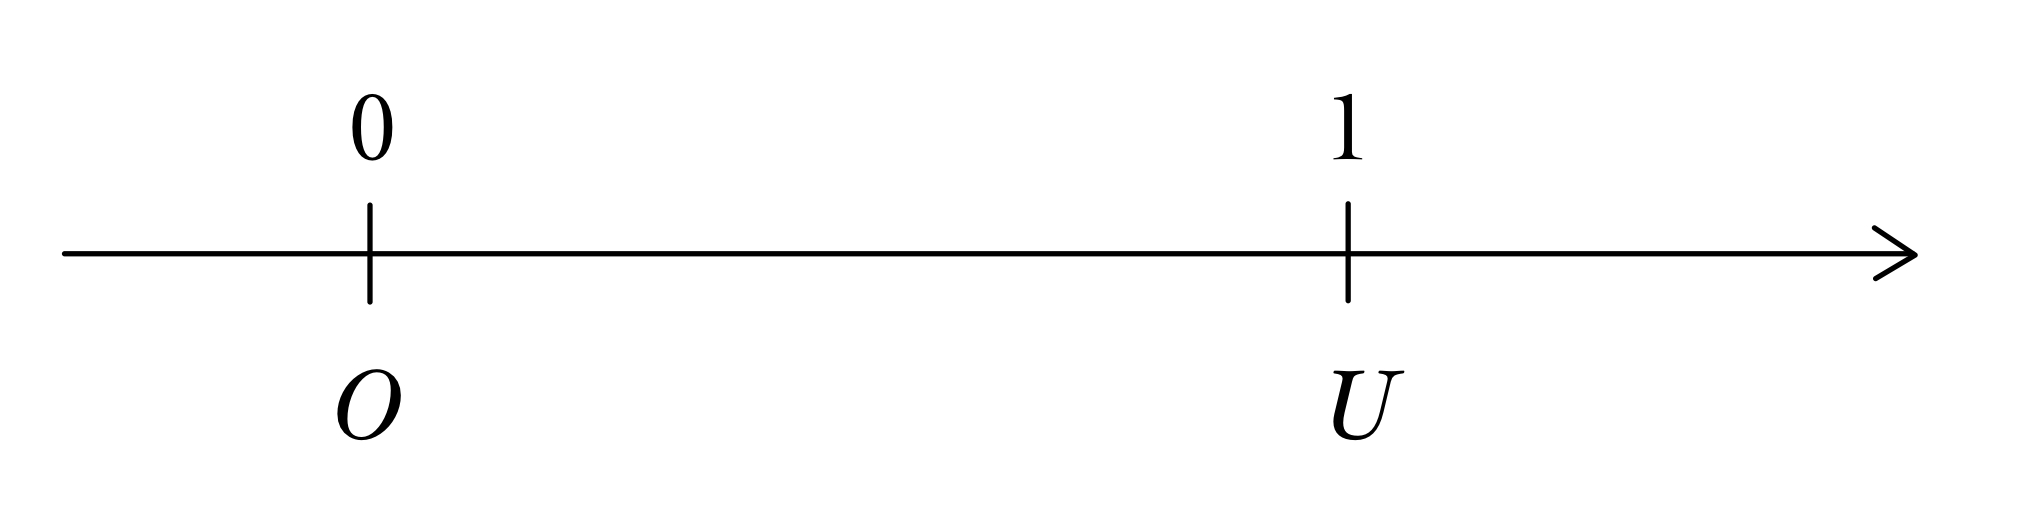
\includegraphics[width=0.5\textwidth]{number_line.PNG}\figtag{1.1.1}
\end{center}

In this manner we establish a one-to-one correspondence between the points of a line and the numbers of the real number system. Figure 1.2.2 shows some real numbers represented as points on the number line. Positive numbers appear to the right of $0$, negative numbers to the left of $0$.

\begin{center}
    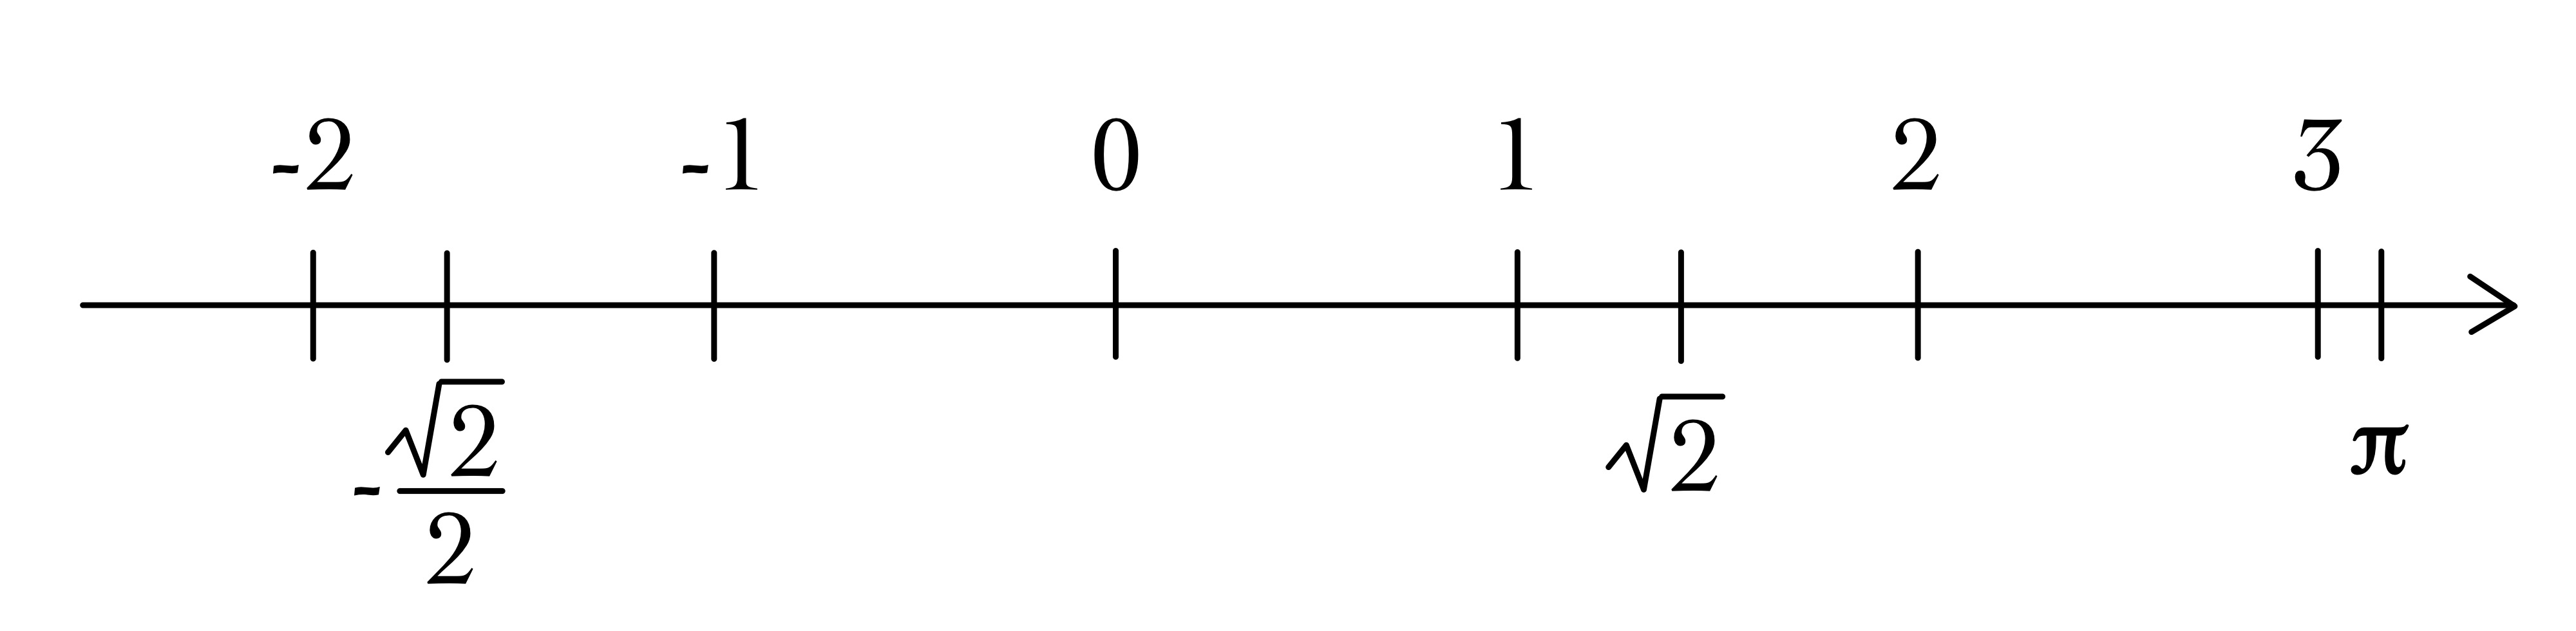
\includegraphics[width=0.65\textwidth]{number_line_example.JPG}\figtag{1.1.2}
\end{center}

\subsection*{Absolute Value}

Let $a\in\bbR$. The symbol $|a|$ is called ``the absolute value of $a$,'' and is defined by \vspace*{0.5em} \begin{equation*}
    |a|=\left\{\begin{array}{rl}a,&\quad\text{if $a\geq0$,}\\-a&\quad\text{if $a<0$.}\end{array}\right.\\[0.5em]
\end{equation*} The geometric meaning of $|a|$ is the distance between $a$ and $0$. Moreover, $|a-b|$ is the distance between $a$ and $b$.

We have some properties regarding the absolute values. 

\begin{theorem}
    Let $a, b\in\bbR$. The following statements always hold.
    \begin{enumerate}
        \item $|a|=0$ if and only if $a=0$.
        \item $|-a|=|a|$.
        \item $|ab|=|a||b|$.
        \item (\textit{Triangle Inequality}) $|a+b|\leq|a|+|b|$.
        \item (\textit{Reverse Triangle Inequality}) $||a|-|b||\leq|a-b|$.
        \item $|a^2|=|a|^2=a^2$.
    \end{enumerate}
\end{theorem}

\subsection*{Interval}

Accurately, intervals are connected subsets in the real number system. We use a pair of parentheses with a comma $(\cdot, \cdot)$ to indicate open intervals and use a pair of brackets with a comma $[\cdot, \cdot]$ to indicate closed intervals.

Suppose $a<b$. The open interval $(a, b)$ is the set of all numbers between $a$ and $b$: $$(a, b)=\{x\in\bbR\mid a<x<b\}.$$
\begin{center}
    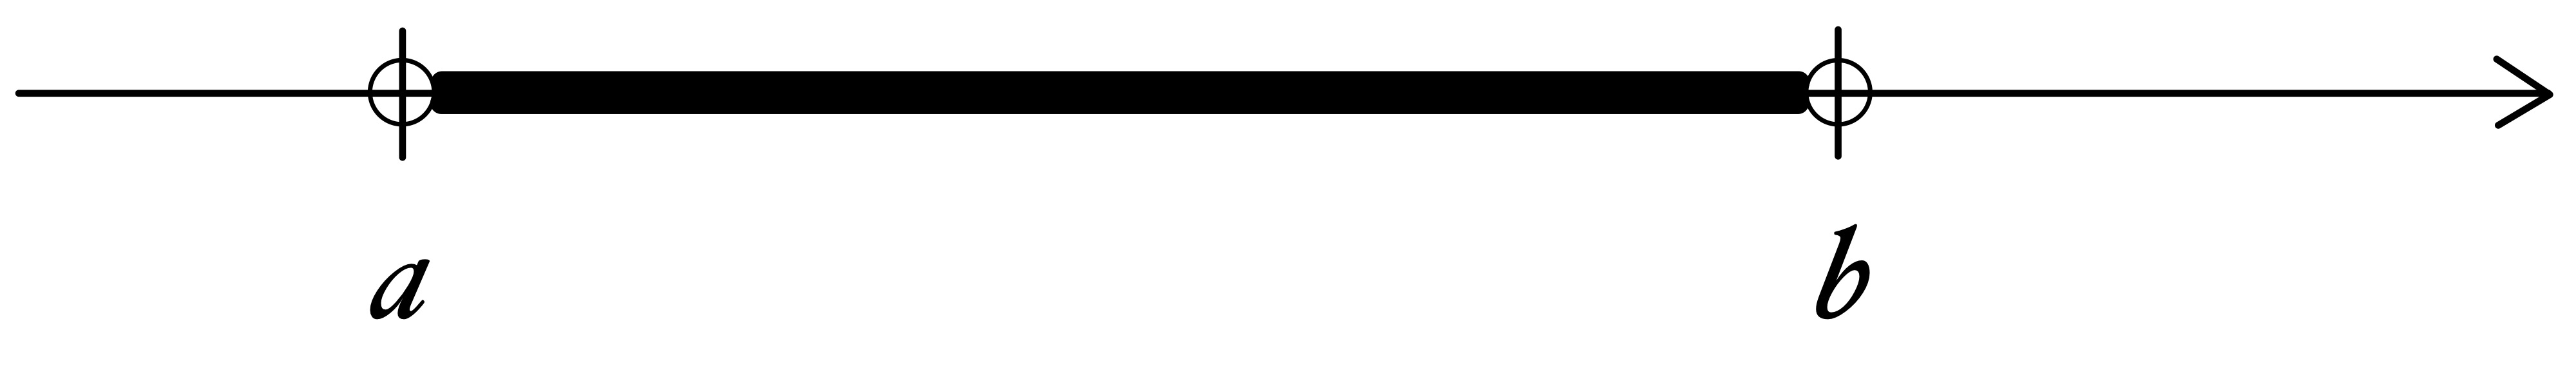
\includegraphics[width=0.45\textwidth]{interval_oo.JPG}
\end{center}
The closed interval $[a, b]$ is the open interval $(a, b)$ with endpoints $a$ and $b$: $$[a, b]=\{x\in\bbR\mid a\leq x\leq b\}.$$
\begin{center}
    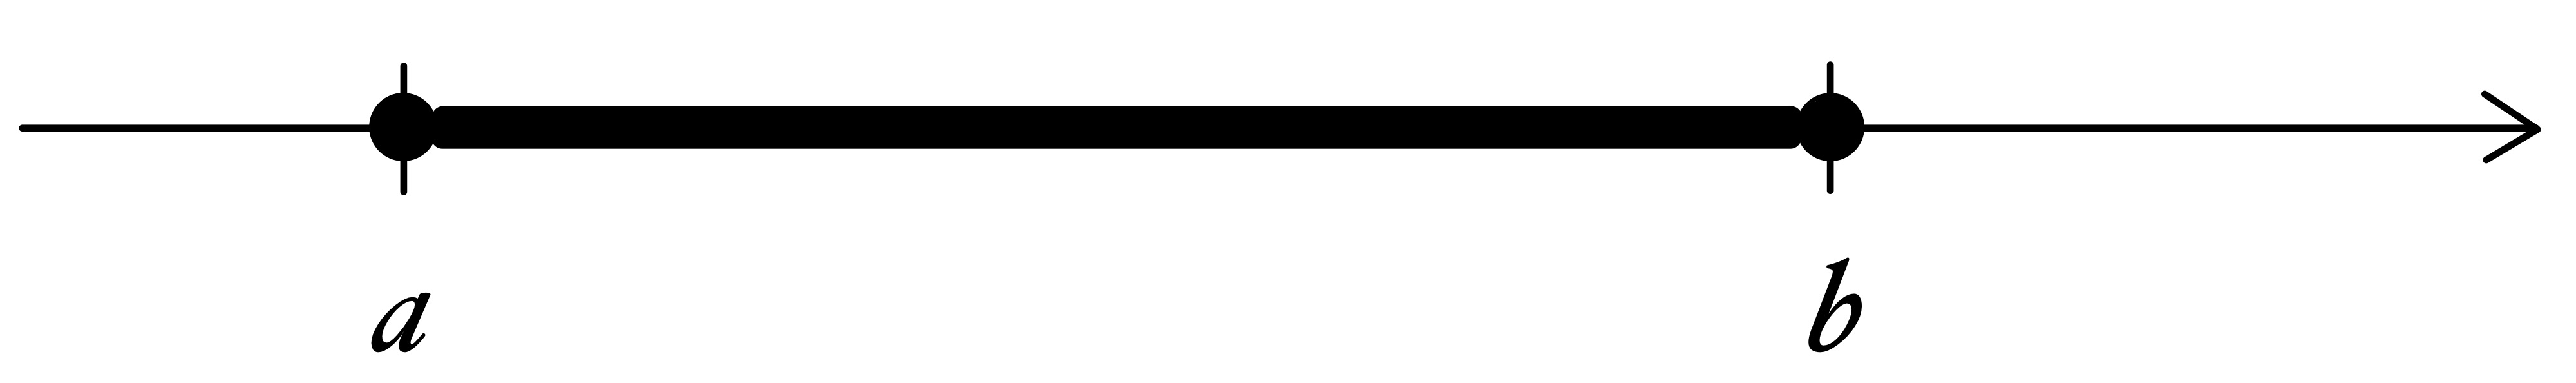
\includegraphics[width=0.45\textwidth]{interval_cc.JPG}
\end{center} We have seven more types of intervals: \begin{align*}
    (a, b]&=\{x\in\bbR\mid a<x\leq b\},\\
    [a, b)&=\{x\in\bbR\mid a\leq x<b\},\\
    (a, \infty)&=\{x\in\bbR\mid x>a\},\\
    [a, \infty)&=\{x\in\bbR\mid x\geq a\},\\
    (-\infty, b)&=\{x\in\bbR\mid x<b\},\\
    (-\infty, b]&=\{x\in\bbR\mid x\leq b\},\\
    (-\infty, \infty)&=\bbR.
\end{align*}

Interval notation is easy to remember: we use a square bracket to include an endpoint and a parenthesis to exclude it. On a number line, inclusion is indicated by a solid dot, exclusion by an open dot. The symbols $\infty$ and $-\infty$, read “infinity” and “negative infinity” (or “minus infinity”), do not represent real numbers. In the intervals listed above, the symbol $\infty$ is used to indicate that the interval extends indefinitely in the positive direction; the symbol $-\infty$ is used to indicate that the interval extends indefinitely in the negative direction.

\subsection*{Basic Algebra}

We use a small number on the top-right of another number to indicate the ``power'', which essentially means the number of multiplication.
\begin{notation}
    Let $r\in\bbR$ and $p\in\bbN\cup\{0\}$. If $p\ne0$, then the number $r^p$ is read ``$r$ to the power $p$'' and is with value $\overbrace{r\times r\times \cdots\times r}^{\text{$p$ times}}$. This explanation only works when the power is a positive integer. If $p=0$ and $r\ne0$, we define $r^0=1$. The number $r$ is called the ``base,'' $p$ is called the ``exponent,'' and $r^p$ is called the ``power.''
\end{notation}

\begin{example}
    By the texts above, we have 
    \begin{enumerate}
        \item $(-2)^2=4$,
        \item $5^4=625$,
        \item $(-1)^5=-1$.
    \end{enumerate}
\end{example}

\begin{notation}
    Let $a>0$ and $p>0$. The number $a^{1/p}$ is called the $p$-th root of $a$ and is the number $b$ such that $b^q=a$; it can also be written as $\sqrt[q]{a}$. If $p=2$, we just write $\sqrt{a}$. The number $a^{-p}$ is the reciprocal of $a^p$.
\end{notation}

We have some special formulas for products and quotients of powers.

\begin{theorem}[Laws of Exponents]
    Let $a>0$ and $p, q\in\mathbb R$. The following always hold.
    \begin{enumerate}
        \item $a^{p+q}=a^p+a^q$.
        \item $a^{p-q}=\dfrac{a^p}{a^q}$.
        \item $(a^p)^q=a^{pq}$.
    \end{enumerate}
\end{theorem}

\begin{example}
    Show that $$a^0=1$$ with the laws of exponents given $a>0$.
\end{example}
\textbf{Proof}. Using $$a^{p-q}=\dfrac{a^p}{a^q},$$ we have 
\begin{align*}
    a^0&=a^{1-1}\\
    &=\dfrac{a^1}{a^1}\\
    &=1,
\end{align*}
which coincides the definition. \qed

Furthermore, we can combine products with summations, factorizing an expression, so that we can find a root more easily.

\begin{theorem}[Factorization]
    Let $a, b\in\bbR$. The following always hold.
    \begin{enumerate}
        \item $(a+b)^2=a^2+2ab+b^2$.
        \item $(a-b)^2=a^2-2ab+b^2$.
        \item $(a+b)^3=a^3+3a^2b+3ab^2+b^3$.
        \item $(a-b)^3=a^3-3a^2b+3ab^2-b^3$.
        \item $a^2-b^2=(a-b)(a+b)$.
        \item $a^3-b^3=(a-b)(a^2+ab+b^2)$.
        \item $a^n-b^n=(a-b)(a^{n-1}+a^{n-2}b+\cdots+ab^{n-2}+b^{n-1})$.
    \end{enumerate}
\end{theorem}

\begin{example}
    Evaluate the following numbers.
    \begin{enumerate}
        \item $255^2-245^2$.
        \item $25+2950+295^2$.
    \end{enumerate}
\end{example}
\textbf{Solution}. For the first number, we use $$a^2-b^2=(a-b)(a+b)$$ with $a=255$ and $b=245$. Hence, $255^2-245^2=10\cdot500=5000$. For the second number, we use $$(a+b)^2=a^2+2ab+b^2,$$ reversely, with $a=5$ and $b=295$. Hence, $25+2950+295^2=(300)^2=90000$. \qed

\begin{example}
    Factorize the following expressions.
    \begin{enumerate}
        \item $x^2-4x+3$.
        \item $x^2+2x-3$.
        \item $x^2+6x+8$.
    \end{enumerate}
\end{example}
\textbf{Solution}. For the first expression, obeserve that $-4=(-3)+(-1)$ and $(-3)\cdot(-1)=+3$. Hence, $$x^2-4x+3=(x-3)(x-1).$$ For the second expression, obeserve that $2=3+(-1)$ and $3\cdot(-1)=-3$. Hence, $$x^2+2x-3=(x+3)(x-1).$$ For the last expression, observe that $6=2+4$ and $2\cdot4=8$. Hence, $$x^2+6x+8=(x+2)(x+4).$$ \qed

Factorization is crucial for solving inequalities and finding roots.

\begin{theorem}[Quadratic Formula]
    Let $a\ne0$, $b, c\in\bbR$. The roots of the equation $$ax^2+bx+c=0$$ are $$x=\dfrac{-b\pm\sqrt{b^2-4ac}}{2a}.$$ The expression $b^2-4ac$ inside the square root is called the ``discriminant'' and is denoted by $D$. If $D>0$, the equation has two distinct real roots. If $D=0$, the equation has one real root. If $D<0$, the equation has two complex roots.
\end{theorem}

\begin{example}
    Solve the equation $$2x^2+3x-2=0.$$
\end{example}
\textbf{Solution}. Using the quadratic formula, $$x=\dfrac{-3\pm\sqrt{3^2+4\cdot2\cdot(-2)}}{2\cdot 2}.$$ Hence, $x=\dfrac{1}{2}$ or $x=-2$. \qed

\subsection*{Exercise}
\begin{enumerate}[label=\arabic*.]
    \item Answer the following questions.
    \begin{enumerate}
        \item We have four people, Anne, Bell, Christine, and Derek, comparing their heights. Suppose Christine is shorter than Anne, Bell is taller than Derek, and Christine is taller than Bell. Arrange them with their heights.
        \item Suppose $a+2=b+20=c-4$. What is the biggest number? What is the smallest number?
    \end{enumerate}
    \item Determine true or false for each of the following statements.
    \begin{enumerate}
        \item $1$ is the smallest positive integer.
        \item $-1$ is the smallest negative integer.
        \item $0$ is an integer.
        \item $1$ is the smallest positive integer.
    \end{enumerate}
    \item Answer the following questions.
    \begin{enumerate}
        \item How many points are there is with unit length $4$ to the origin?
        \item Evaluate the following expressions.
        \begin{enumerate}[label=\alph*.]
            \item $|-5|-|8|$.
            \item $|-3-7|$.
            \item $|5-\sqrt{5}|$.
            \item $|2-\pi|$.
        \end{enumerate}
        \item Does the equation $\sqrt{a^2}=a$ hold for all $a\in\bbR$?
        \item Suppose moving $6$ meters to the right of the origin can be denoted as $+2$. How can moving $15$ meters to the left of the origin be denoted?
        \item There are three points $A$, $B$, and $C$ on the number line, with coordinate $1$, $6$, and $8$, respectively. Suppose one set the origin to $B$ without changing the unit length. What is the coordinate of $A$? What is the coordinate of $C$?
        \item If $a-b=18$ and $|a|=|b|$, what are $a$ and $b$?
        \item If $a$ and $b$ are with different signs, i.e., $ab<0$, and $|a|=|b|$, what is the value of $a+b$?
        \item Suppose $a$ and $b$ are all negative. If $|a|>|b|$, what is the order between $a$ and $b$?
    \end{enumerate}
    \item Answer the following questions.
    \begin{enumerate}
        \item If $3|a+2|+2|b-7|=0$, what are $a$ and $b$?
        \item If $|4-a|=1$, what is $a$?
        \item If $a>0$, what is $|a|$?
        \item If $a<0$, what is $|a|$?
        \item How many integers $a$ are there satisfying $4<|a|<7$?
        \item How many integers $c$ are there satisfying $|c|\leq 4$?
        \item If $|a-2|=2$, what is $a$?
        \item If $|c+2|=8$, what is $c$?
    \end{enumerate}
    \item Answer the following questions.
    \begin{enumerate}
        \item What is $[0, 2]\cap(2, 4)$?
        \item What is $[0, 1]\setminus(0, \infty)$?
        \item What is the interval $I$ such that only elements $x$ in $I$ suffice $|x|\leq 3$?
        \item What is the interval $J$ such that only elements $x$ in $J$ suffice $x^2<16$?
    \end{enumerate}
    \item Answer the following questions.
    \begin{enumerate}
        \item If $25^{3m}=3$ and $5^{7n}=\dfrac{1}{3}$, what is the value of $(6m+7n-2)^5$?
        \item If $8^{2a}=4$, what is the value of $8^{6a}$?
        \item If $x^{2a}=3$, what is the value of $\dfrac{x^{3a}-x^{-a}}{x^{3a}+x^{-a}}$?
        \item If $a\cdot567^3=10^3$ and $\dfrac{a}{10^3}=b$, what is the value of $a\cdot b$?
    \end{enumerate}
    \item Factorize the following expressions.
    \begin{enumerate}
        \item $x(b-c)-y(c-b)$.
        \item $(x-a)(x+3)+(3-x)(x-b)$.
        \item $(x^2+6x)^2-9^2$.
        \item $(x^2+3x)^-(x+4)^2$.
        \item $x^2+4x+4-y^2$
    \end{enumerate}
    \item Find the real roots of the equation.
    \begin{enumerate}
        \item $x^2-x-2=0$.
        \item $x^2-9=0$.
        \item $x^2-6x+9=0$.
        \item $x^2+8x+16=0$.
        \item $x^2-2x+5=0$.
        \item $(x-3)^2-16=0$.
    \end{enumerate}
\end{enumerate}

\section{Inequalities}

Inequalities can be similarly solved like one solving an equation, adding the same number to both sides or by multiplying both sides by the same positive number. The relation will be reversed when multiplied both sides by the same negative number.

\begin{example}
    Solve the inequality $$-4(3-x)\leq 12.$$
\end{example}
\textbf{Solution}. Multiplying both sides by $\dfrac{1}{4}$, we have $$x-3\leq 3.$$ Adding $3$ to both sides, we have $$x\leq 6.$$ Hence, the solution set is the interval $(-\infty, 6]$. \qed

\begin{example}
    Solve the inequality $$x^2-4x+3>0.$$
\end{example}
\textbf{Solution}. Factorizing the expression on the left, we have $$(x-3)(x-1)>0.$$ The inequality only holds when the expression $(x-3)$ and the expression $(x-1)$ are with the same sign. That is, the inquality only holds when \begin{enumerate}
    \item $x-3>0$ and $x-1>0$, or
    \item $x-3<0$ and $x-1<0$.
\end{enumerate}
For the first scenario, $(3, \infty)$ is the set of solutions. For the second scenario, $(-\infty, 1)$ is the set of solutions. Hence, the set of solutions for the inequality is $(-\infty, 1)\cup(3, \infty)$. \qed

\begin{example}
    Solve the inequality $$|x+2|<3.$$
\end{example}
\textbf{Solution}. Using the geometric meaning of the absolute value, the set of solutions is the set containing points with distance less than $3$ to point $-2$. Hence, the set of solutions is $(-5, 1)$. \qed\\
\textbf{Alternative Solution}. We can write $$|x+2|<3$$ as $$-3<x+2<3.$$ Adding $-2$ to each expression of the inequalities, we have $$-5<x<1.$$ \qed

\begin{theorem}[Triangle inquality]
    Let $a, b\in\bbR$. The inequality $$|a+b|\leq |a|+|b|$$ must hold.
\end{theorem}
\textbf{Proof}. We have the natural equality $2ab\leq2|ab|$. Adding $a^2+b^2$ to both sides, we have $$a^2+2ab+b^2\leq |a|^2+2|a||b|+|b|^2.$$ Since both sides are non-negative, taking square roots yeilds $$|a+b|\leq |a|+|b|.$$ \qed

\subsection*{Exercise}
\begin{enumerate}[label=\arabic*.]
    \item Solve the following inqualities. Afterwards, express the solution set as an interval or as the union of intervals and mark the solution set on a number line.
    \begin{enumerate}
        \item $2+3x<5$.
        \item $16x+64\leq16$.
        \item $7x(x-4)^2<0$.
        \item $|x|<2$.
        \item $0<|x|<1$.
        \item $|3x+1|>5$.
    \end{enumerate}
    \item Each of the following sets is the solution of an inequality of the form $|x-c|<\delta$. Find $c$ and $\delta$.
    \begin{enumerate}
        \item $(-3, 3)$.
        \item $(-3, 7)$.
        \item $(-7, 3)$
        \item $(0, 4)$.
        \item $(a, b)$.
    \end{enumerate}
    \item Given that $x>1$, arrange the following in order: $$1, x, \sqrt{x}, \dfrac{1}{x}, \dfrac{1}{\sqrt{x}}.$$
    \item Given that $0<x<1$, arrange the following in order: $$1, x, \sqrt{x}, \dfrac{1}{x}, \dfrac{1}{\sqrt{x}}.$$
\end{enumerate}

\section{Functions}

Functions can be imagined as a black box. You throw a parameter $x$ into the black box $f$, and then you obtain the result $f(x)$. Mathematically speaking, a function is a correspondence between two sets, domain and range. For example, a teacher is marking exams for students. There are twenty questions in total. A student gets five points with a correct answer to a question. In this case, the score is a function of the number of correct answers. In mathematical language, we say the score is $f_{\text{score}}(x)=5x$, where $x$ is the number of correct answers. Since the number of correct answers can only be positive integers among $0$ and $20$, we say the domain (the set where the function is valid) is $\{0, 1, 2, \dots, 19, 20\}$. The range, the set with all positive outcomes for the function, is $\{0, 5, 10, \dots, 95, 100\}$ in this case.

To be more specific, we use a colon ``$:$'' and an arrow ``$\to$'' to indicate the function and its domain and codomain (a set that contains the range). One generally indicates codomain since one does not know exactly the range is. For example, I can write $f_{\text{score}}:\{0, 1, 2, \dots, 19, 20\}\to\bbN$, which indicates that the domain of the function $f_{\text{score}}$ is $\{0, 1, 2, \dots, 19, 20\}$, and all the outputs will be in $\bbN$.

Take another familiar example, the square function $f_{\text{square}}$. The square function outputs the square of an input. Since you can square any real numbers, we write $f_{\text{square}}:\bbR\to\bbR$ with $f(x)=x^2$ for all $x\in\bbR$, or more specificly, $f_{\text{square}}:\bbR\to\bbR_{\geq0}$ with $f(x)=x^2$ for all $x\in\bbR$. One can use the arrow with a small stroke on the left ``$\mapsto$'' to indicate the way of mapping. For example, $x\mapsto x^2$ is the square function. We are familiar with the absolute value. In fact, the absolute value is a function with domain $\bbR$ and range $[0, \infty)$.

Usually, we call the input $x$ the independent variable (or argument), and we call the output $y$ the dependent variable, since $y$ varies on $x$.

\begin{definition}[Injective, Surjective, and Bijective]
    A function $f:X\to Y$ is \underline{injective} if $x_1\ne x_2\in X$ implies $f(x_1)\ne f(x_2)$. A function $g:X\to Y$ is \underline{surjective} if there exists a $x\in X$ such that $f(x)=y$ for all $y\in Y$. A function is bijective if it is surjective and injective.
\end{definition}

\begin{definition}[Graph]
    Let $f:X\to Y$ be a function. The \underline{graph} of $f$ is the set $$\{(x, y)\mid x\in X\text{ and }y=f(x)\}.$$
\end{definition}

\subsection*{Symmetry}

\begin{definition}[Even and Odd]
    A function $f:X\to Y$ is said to be \underline{even} if $f(x)=f(-x)$ for all $x\in X$. A function $g:X\to Y$ is said to be \underline{odd} if $f(x)=g(-x)$ for all $x\in X$.
\end{definition}

Functions in both genres are all called ``symmetric'' since an even function is symmetric from the $y$-axis, and an odd function is symmetric from the origin.

\begin{example}
    Determine whether the following functions are even, odd, or neither.
    \begin{enumerate}
        \item $f_1(x)=x$.
        \item $f_2(x)=x+1$.
        \item $f_3(x)=|x|$.
        \item $f_4(x)=x^2$.
        \item $f_5(x)=x^3$.
        \item $f_6(x)=2^x+2^{-x}$.
    \end{enumerate}
\end{example}
\textbf{Solution}. The function $f_1$ is odd since $f_1(x)=x=-f_1(x)=-(-x)$. The function $f_2$ is neither even nor odd. The function $f_3$ is even since $|x|=|-x|$. The function $f_4$ is also even. The function $f_5$ is odd. The function $f_6$ is even since $f_6(x)=2^x+2^{-x}=f_6(-x)=2^{-x}+2^x$. \qed

\subsection*{Exercise}

\begin{enumerate}[label=\arabic*.]
    \item Calculate $f(0), f(1), f(-1)$ with the following functions.
    \begin{enumerate}
        \item $f(x)=|x|$.
        \item $f(x)=2x^2-3x+2$.
        \item $f(x)=\dfrac{2x-1}{x^2+4}$.
        \item $f(x)=\sqrt{x^2+2x+5}$.
        \item $f(x)=|x+3|-5x$.
    \end{enumerate}
    \item Calculate $f(a), f(-a), f(a+h), \dfrac{f(a+h)-f(a)}{h}$ with the following functions.
    \begin{enumerate}
        \item $f(x)=x^2-2x$.
        \item $f(x)=2x^2-3x$.
        \item $f(x)=\dfrac{1}{x-2}$.
    \end{enumerate}
    \item Give the domain and range of the function.
    \begin{enumerate}
        \item $f(x)=|x|$.
        \item $f(x)=\dfrac{1}{x^2}$.
        \item $f(x)=\sqrt{x-3}$.
        \item $f(x)=\dfrac{1}{\sqrt{2-x}}$.
    \end{enumerate}
    \item Give the domain and range of the function and sketch the graph of the function.
    \begin{enumerate}
        \item $f(x)=1$.
        \item $f(x)=-1$.
        \item $f(x)=2x$.
        \item $f(x)=2x+1$.
        \item $f(x)=|x-1|$.
        \item $f(x)=\left\{\begin{array}{rl}
            -1,\quad&\text{if $x<0$,}\\1,\quad&\text{if $x>0$}.
        \end{array}\right.$
    \end{enumerate}
    \item Determin whether the following functions are even, odd, or neither.
    \begin{enumerate}
        \item $f(x)=x^2+1$.
        \item $f(x)=\dfrac{x^2}{1-|x|}$.
        \item $f(x)=x+\dfrac{1}{x}$.
        \item $f(x)=\sqrt[5]{x-x^3}$.
    \end{enumerate}
\end{enumerate}

\section{Elementary Functions}

The functions that figure most prominently in single-variable calculus are the polynomial functions, the rational functions, the trigonometric functions, the exponential functions, and the logarithmic functions. These functions are generally known as the elementary functions.

\subsection*{Polynomial Functions}

\begin{definition}[Polynomial]
    Let $n\in\bbN\cup\{0\}$. An expression of the form $$a_nx^n+a_{n-1}x^{n-1}+\cdots+a_1x+a_0$$ with $a_i\in\bbR$, $i=0, 1, \dots, n$, is a \underline{polynomial}. This is called a real polynomial of degree $n$.
\end{definition}

\begin{example}
    The following are polynomials.
    \begin{enumerate}
        \item $x^2+x+1$.
        \item $-\pi x^4-7$.
        \item $x^{256}$.
        \item $0$.
    \end{enumerate}
\end{example}

\begin{example}
    The following are \textbf{NOT} polynomials.
    \begin{enumerate}
        \item $x+1+\dfrac{1}{x}$.
        \item $|x|+5$.
        \item $\sqrt{2x}-7$.
    \end{enumerate}
\end{example}

\begin{definition}[Polynomial Function]
    A \underline{polynomial function} $P$ is a function with output a polynomial, i.e., $P(x)=a_nx^n+a_{n-1}x^{n-1}+\cdots+a_1x+a_0$.
\end{definition}

\begin{theorem}[Fundamental Theorem of Algebra]
    Every single-variable real polynomial of degree $n$ has exactly $n$ complex roots counted with multiplicity.
\end{theorem}

\subsection*{Rational Functions}

\begin{definition}[Rational Function]
    A \underline{rational function} is the quotient of two polynomial functions, i.e., $R(x)=\dfrac{P_1(x)}{P_2(x)}$.
\end{definition}

A rational function will have a vertical asymptote at $x=a$ such that $P_2(a)=0$. For example, the function $f(x)=\dfrac{1}{x}$ has a vertical asymptote at $x=0$. See Figure 1.4.1.

\begin{example}
    Find vertical asymptotes of the following functions.
    \begin{enumerate}
        \item $f_1(x)=\dfrac{1}{x^2+4x+4}$.
        \item $f_2(x)=\dfrac{1}{x^2-1}$.
    \end{enumerate}
\end{example}
\textbf{Solution}. For function $f_1$, since $x^2+4x+4=(x+2)^2$, the vertical asymptote is $x=-2$. For function $f_2$, since $x^2-1=(x+1)(x-1)$, the vertical asymptotes are $x=1$ and $x=-1$. \qed

\begin{center}
    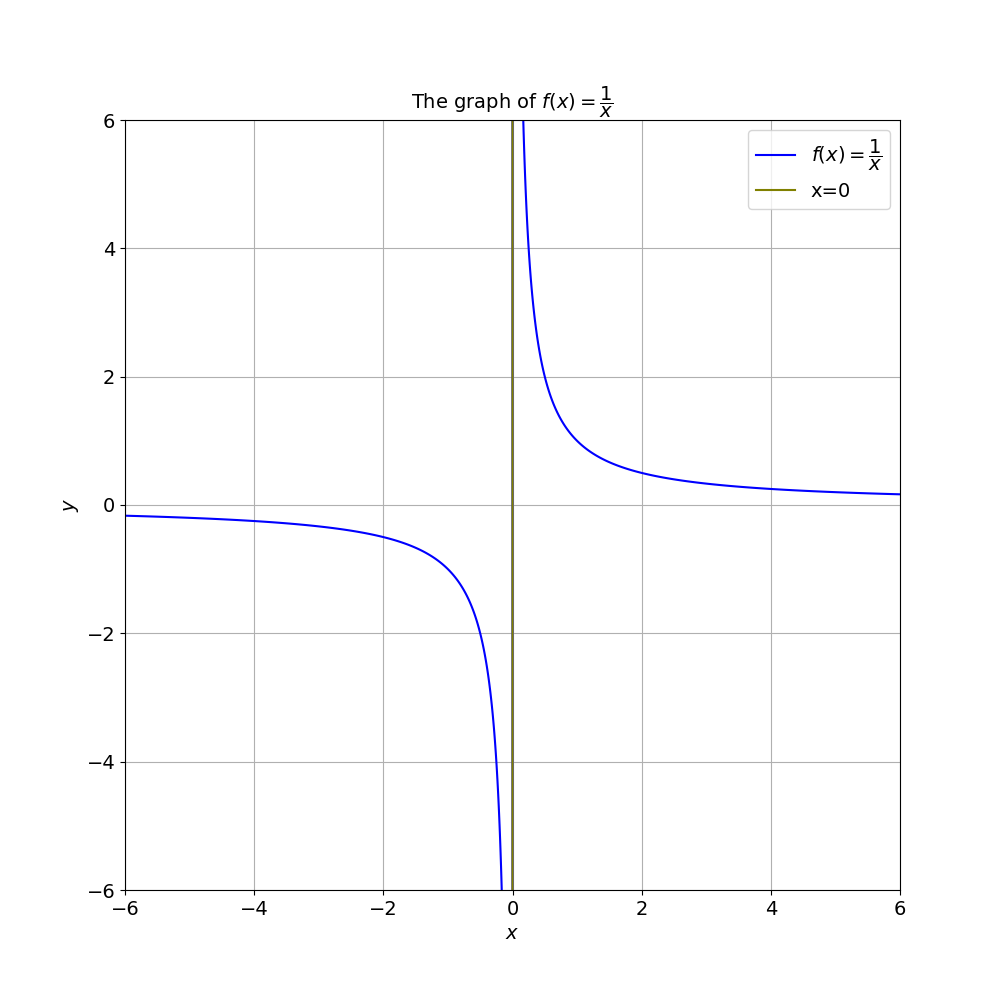
\includegraphics[width=0.5\textwidth]{reciprocal_of_x.png}\figtag{1.4.1}
\end{center}

\subsection*{Trigonometric Functions}

Trigonometric functions are originally the ratio between sides of a right triangle. For example, if I have a triangle with lengths $a, b, c$ and an angle $\theta$.

\begin{center}
    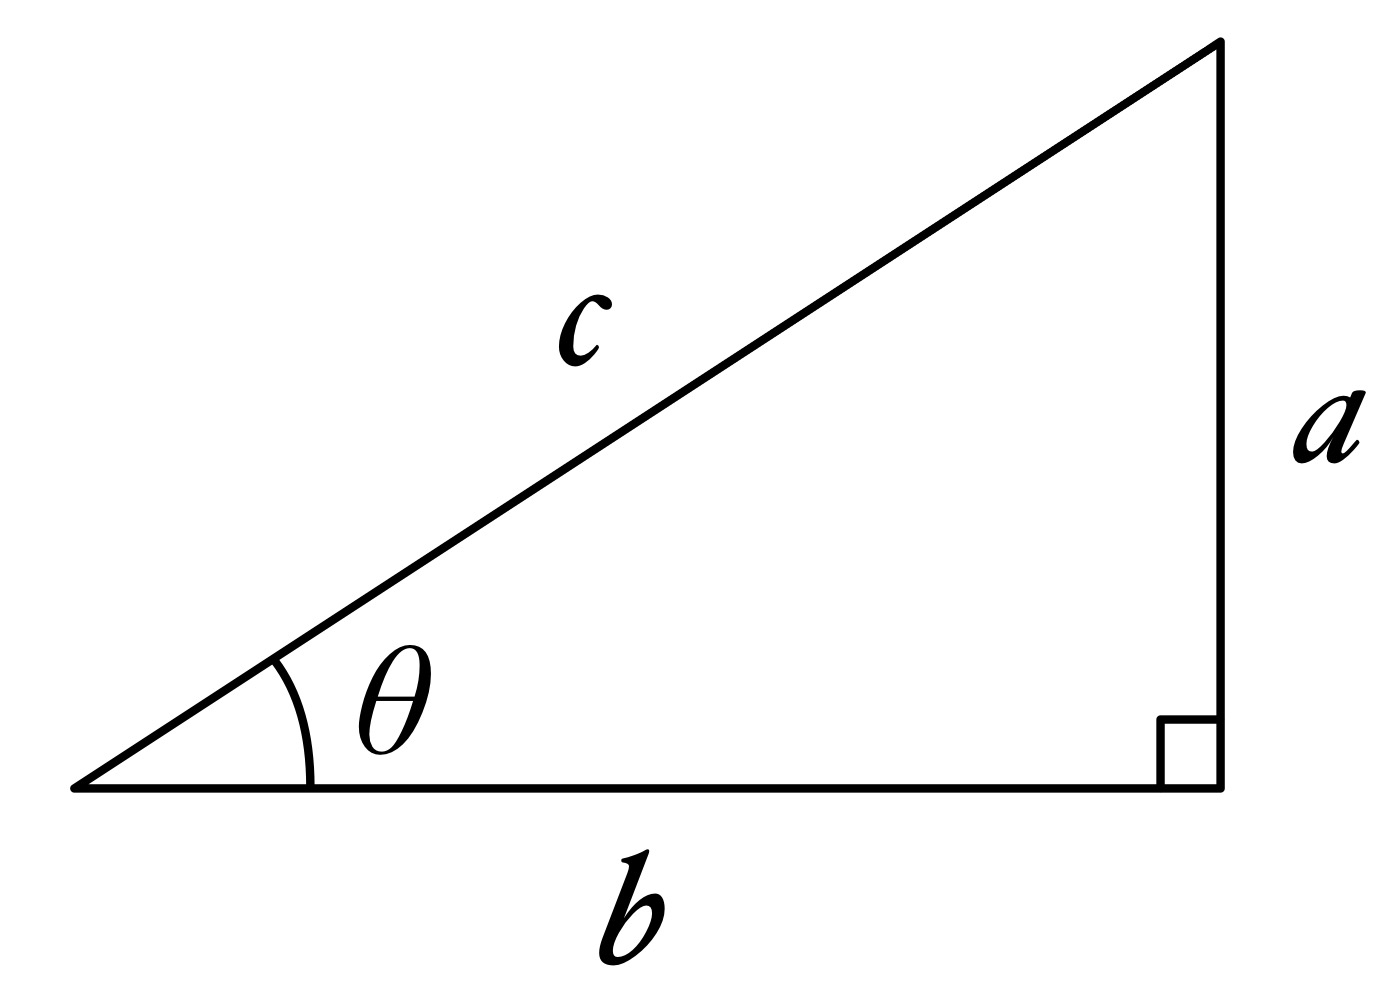
\includegraphics[width=0.2\textwidth]{triangle.JPG}\figtag{1.4.2}
\end{center}

The ratio $\dfrac{a}{c}$ of the length of the hypotenuse $c$ to the length of the opposite leg $a$ is called $\sin\theta$. The ratio $\dfrac{b}{c}$ of the length of the hypotenuse $c$ to the length of the adjecent leg $b$ is called $\cos\theta$. The ratio $\dfrac{\sin\theta}{\cos\theta}$ is called $\tan\theta$, is also the ratio of the length of the adjecent leg $b$ to the length of the opposite leg $a$.

\subsubsection*{Radian Measure}

Degree measure, traditionally used to measure angles, has a serious
drawback. It is artificial; there is no intrinsic connection between a degree and the geometry of a rotation. Why choose $360^\circ$ for one complete revolution? Why not $100^\circ$ or $400^\circ$? There is another way of measuring angles that is more natural and lends itself better to the methods of calculus: measuring angles in radians.

We first introduce $\pi$, the ratio of the length of a half circumference of a circle to the length diameter of the circle. Since a hald circumference is just a half circle, we say that $\pi\ \text{rad}$ is $180^\circ$. Hence, $2\pi\ \text{rad}$ is $360^\circ$. The following table gives some common angles (rotations) measured both in degrees and in radians.

\begin{center}
    \begin{tabular}{|cccccccccccc|}
        \hline
        degrees & $0^\circ$ & $30^\circ$ & $45^\circ$ & $60^\circ$ & $90^\circ$ & $120^\circ$ & $135^\circ$ & $150^\circ$ & $180^\circ$ & $270^\circ$ & $360^\circ$\\
        \hline
        radians & $0$ & $\dfrac{1}{6}\pi$ & $\dfrac{1}{4}\pi$ & $\dfrac{1}{3}\pi$ & $\dfrac{1}{2}\pi$ & $\dfrac{2}{3}\pi$ & $\dfrac{3}{4}\pi$ & $\dfrac{5}{6}\pi$ & $\pi$ & $\dfrac{3}{2}\pi$ & $2\pi$\\[0.2em]
        \hline
    \end{tabular}
\end{center}

\subsubsection*{Sine and Cosine}

Let $\theta$ be any real number. The rotation $\theta$ takes the point $A$ with coordinates $(1, 0)$ to some point $P$, also on the unit circle. The coordinates of $P$ are completely determined by $\theta$ and have names related to $\theta$. The second coordinate of $P$ is $\sin\theta$, and the first coordinate of $P$ is $\cos\theta$. Figure 1.4.3 illustrates the idea. To simplify the diagram, we have taken $\theta$ from $0$ to $2\pi$.

For each real $\theta$, the rotation $\theta$ and the rotation $\theta+2\pi$ take the point $A$ to exactly the same point $P$. If follows that for each $\theta$, $$\sin(\theta+2\pi)=\sin\theta\qquad\text{and}\qquad\cos(\theta+2\pi)=\cos\theta.$$

\begin{center}
    \begin{minipage}{0.48\textwidth}
        \begin{center}
            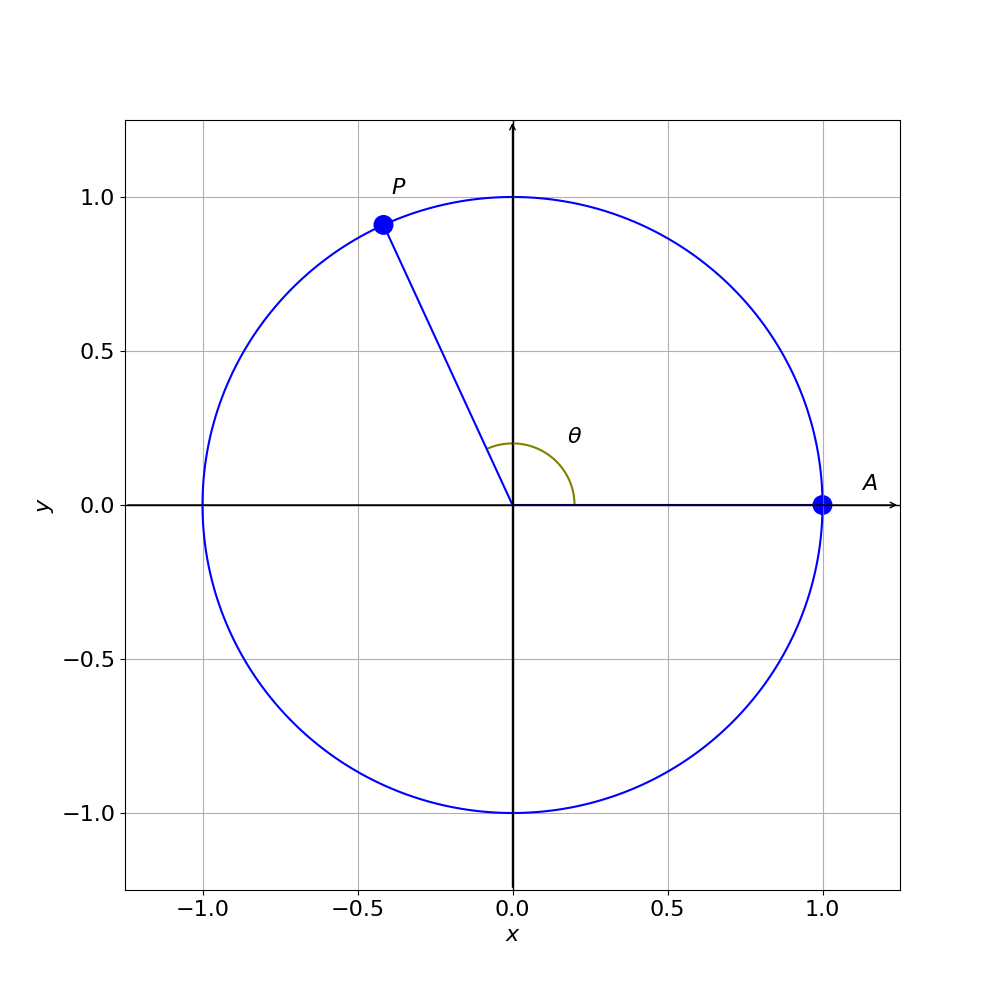
\includegraphics[width=0.85\textwidth]{unit_circle_1.png}\figtag{1.4.3}
        \end{center}
    \end{minipage}
    \begin{minipage}{0.48\textwidth}
        \begin{center}
            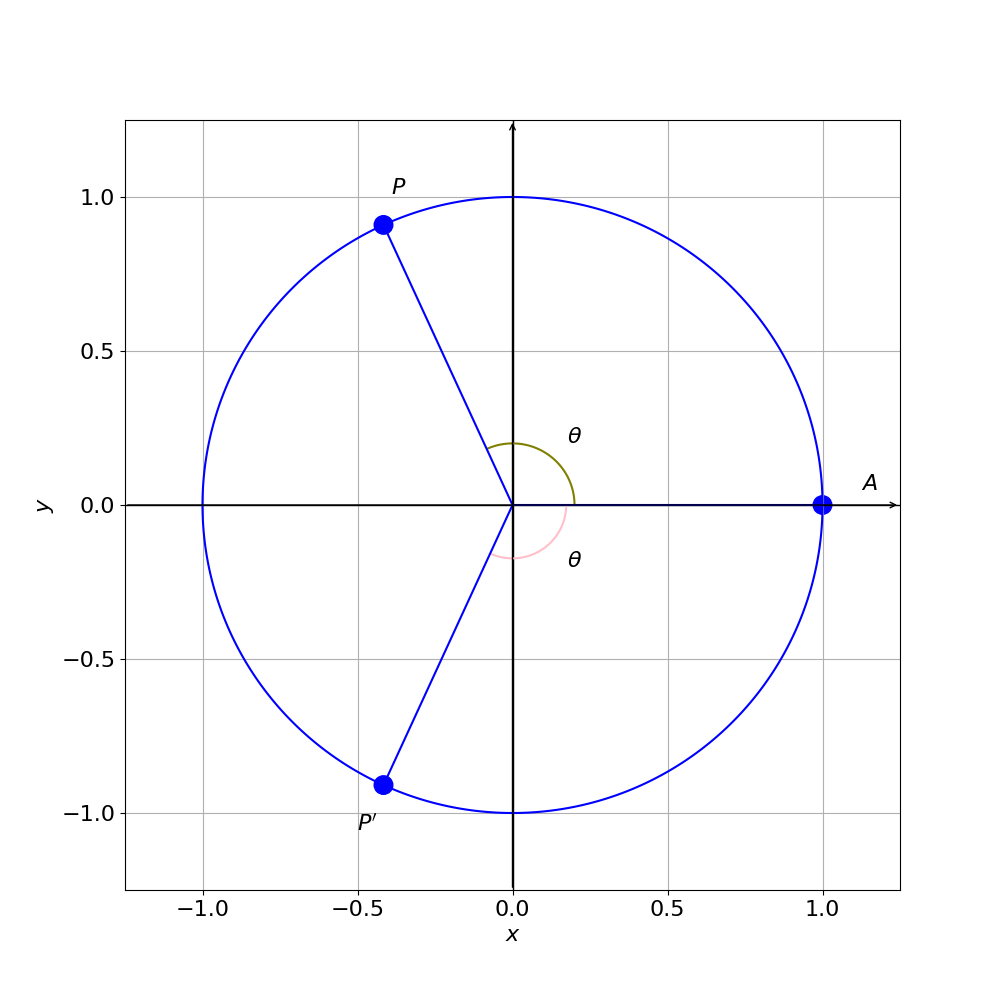
\includegraphics[width=0.85\textwidth]{unit_circle_2.png}\figtag{1.4.4}
        \end{center}
    \end{minipage}
\end{center}

\vspace*{1.5em}

A rotation of $\pi\ \text{rad}$ takes each point to the point antipodal to it: $(x, y)\mapsto(-x, -y)$. Thus, $$\sin(\theta+\pi)=-\sin\theta\qquad\text{and}\qquad\cos(\theta+\pi)=-\cos\theta.$$

In Figure 1.4.4, we consider two rotations, a positive rotation $\theta$ and its negative counterpart $-\theta$, from point $A$ respectively to point $P$ and to point $P'$. From the figure, you can see that $$\sin(-\theta)=-\sin\theta\qquad\text{and}\qquad\cos(-\theta)=\cos\theta.$$

\subsubsection*{Tangent, Cotangent, Secant, Cosecant}

We have four more trigonometric functions: the tangent, the cotangent, the secant, the cosecant. These are obtained as follows: $$\tan\theta=\dfrac{\sin\theta}{\cos\theta},\qquad\cot\theta=\dfrac{\cos\theta}{\sin\theta},\qquad\sec\theta=\dfrac{1}{\cos\theta},\qquad\text{and}\qquad\csc\theta=\dfrac{1}{\sin\theta}.$$ Note that the tangent function is an odd function, $$\tan(-\theta)=\dfrac{\sin(-\theta)}{\cos(-\theta)}=\dfrac{-\sin\theta}{\cos\theta}=-\tan\theta.$$

\subsubsection*{Identities}

\begin{theorem}[Trigonometric Identity]
    Let $\theta, \alpha, \beta\in\bbR$. The following always hold.
    \begin{enumerate}
        \item $(\sin\theta)^2+(\cos\theta)^2=1, \qquad (\tan\theta)^2+1=(\sec\theta)^2,\qquad 1+(\cot\theta)^2=(\csc\theta)^2$.
        \item $\sin(\theta+2\pi)=\sin\theta,\qquad\cos(\theta+2\pi)=\cos\theta,\qquad\tan(\theta+\pi)=\tan\theta$.
        \item $\sin(-\theta)=-\sin\theta,\qquad\cos(-\theta)=\cos\theta,\qquad\tan(-\theta)=-\tan(\theta)$.
        \item $\sin(\alpha+\beta)=\sin\alpha\cos\beta+\cos\alpha\sin\beta,\qquad\cos(\alpha+\beta)=\cos\alpha\cos\beta-\sin\alpha\sin\beta$.
    \end{enumerate}
\end{theorem}

\subsection*{Exponential Functions and Logarithmic Function}

\begin{definition}[Exponential Function]
    Let $a>0$ with $a\ne1$. Let $f:\bbR\to\bbR^+$ be a function defined by $f(x)=a^x$. The function $f$ is called an \underline{exponential function} with base $a$.
\end{definition}

\begin{definition}[Logarithmic Function]
    Let $b>0$ with $b\ne 1$. Let $g:\bbR^+\to\bbR$ be defined by $b^{g(x)}=x$. Then $g(x)$ is well-defined function and is called a \underline{logarithmic function}. The function $g$ is denoted by $\log_b$.
\end{definition}

\begin{theorem}
    Let $a>0$ with $a\ne 0$. Then, $a^{\log_a(x)}=x$. That is, the exponential function and the logarithmic function are inverse functions.
\end{theorem}

\subsection*{Exercise}

\begin{enumerate}[label=\arabic*.]
    \item State whether the function is a polynomial function, a rational function, or neither. If it is a polynomial function, give the degree.
    \begin{enumerate}
        \item $f(x)=3$.
        \item $f(x)=-x^{-1}$.
        \item $f(x)=\dfrac{x^2-4}{\sqrt{2}}$.
        \item $f(x)=\dfrac{x^2-2x-8}{x+2}$.
        \item $f(x)=\dfrac{(\sqrt{x}+2)(\sqrt{x}-2)}{x^2+4}$.
        \item $f(x)=\dfrac{1}{x^2-4}$.
        \item $f(x)=x+\dfrac{1}{x}$.
    \end{enumerate}
    \item Convert the degree measure into radian measure.
    \begin{enumerate}
        \item $225^\circ$.
        \item $-210^\circ$.
        \item $450^\circ$.
        \item $1^\circ$.
    \end{enumerate}
    \item Convert the radian measure into degree measure.
    \begin{enumerate}
        \item $-3\pi/2$.
        \item $5\pi/4$.
        \item $2$.
        \item $-\sqrt{3}$.
    \end{enumerate}
    \item Compute $\sin\theta$ and $\cos\theta$ with $\theta=0, \dfrac{\pi}{6}, \dfrac{\pi}{4}, \dfrac{\pi}{3}, \dfrac{\pi}{2}, \dfrac{2\pi}{3}, \dfrac{3\pi}{4}, \pi.$
    
\end{enumerate}


\section{Operations on Functions}

\setlength{\delimitershortfall}{0pt}

Just like numbers, we can add functions $$(f+g)(x)=f(x)+g(x),$$ multiply functions $$(fg)(x)=f(x)\cdot g(x),$$ and divide functions $$\left(\dfrac{f}{g}\right)(x)=\dfrac{f(x)}{g(x)}$$ given that $g(x)\ne 0$. We can also multiply a function $f$ by a real number $\alpha$ $$(\alpha f)(x)=\alpha\cdot f(x).$$

\setlength{\delimitershortfall}{13.5pt}

\begin{example}
    Let $f(x)=\sqrt{x+3}$ and $g(x)=\sqrt{5-x}-2$.
    \begin{enumerate}
        \item Determine the domain of $f$, of $g$, and of $f+g$.
        \item Specify $(f+g)(x)$.
    \end{enumerate}
\end{example}
\textbf{Solution}. Note that the number in the square root cannot be less than zero. The domain of $f$ is $[-3, \infty)$, and the one of $g$ is $(-\infty, 5]$. Hence, the domain of $f+g$ is $[-3, \infty)\cap(-\infty, 5]=[-3, 5]$. The function $(f+g):[-3, 5]\to\bbR$ is defined by $(f+g)(x)=\sqrt{x+3}+\sqrt{5-x}-2$. \qed

Aside from the operations you already knew, there is a new operation, called ``composition.''

\begin{definition}[Composition]
    Let $f:\tilde{X}\to X$ and $g:X\to Y$. We define the \underline{composition} of $f$ with $g$, denoted by $f\circ g$, by $(f\circ g)(x)=f(g(x))$.
\end{definition}

\begin{example}
    Find $(f_i\circ g_i)(x)$ and $(g_i\circ f_i)(x)$ for the following functions.
    \begin{enumerate}
        \item $f_1(x)=x^2, \quad g_1(x)=\sin x$.
        \item $f_2(x)=x^2-1, \quad g_2(x)=\sqrt{3-x}$.
    \end{enumerate}
\end{example}
\textbf{Solution}. For the first pair of functions, $(f_1\circ g_1)(x)=(\sin x)^2$ and $(g_1\circ f_1)(x)=\sin(x^2)$. For the second pair, $(f_2\circ g_2)(x)=|x-3|-1$ and $(g_2\circ f_2)(x)=\sqrt{4-x^2}$. \qed

Note that the domain and range will change after composition.

\subsection*{Exercise}

\setlength{\delimitershortfall}{0pt}

\begin{enumerate}[label=\arabic*.]
    \item Let $f(x)=x+\dfrac{1}{\sqrt{x}}$ and $g(x)=-\sqrt{x}$. Find the following function.
    \begin{enumerate}
        \item $2f$.
        \item $6f$.
        \item $3g$.
        \item $6f+3g$.
        \item $f-g$.
        \item $fg$.
    \end{enumerate}
    \item Suppose $f$ and $g$ are odd. What can you conclude about $fg$?
    \item Suppose $f$ and $g$ are even. What can you conclude about $fg$?
    \item Given a function $f:\bbR\to\bbR$. Show that the function $g(x)=f(x)+f(-x)$ is even.
    \item Given a function $f:\bbR\to\bbR$. Show that the function $h(x)=f(x)-f(-x)$ is even.
    \item Find $f$ such that $f\circ g=F$ for the following functions.
    \begin{enumerate}
        \item $g(x)=\dfrac{1+x^2}{1+x^4}, \quad F(x)=\dfrac{1+x^4}{1+x^2}$.
        \item $g(x)=x^2, \quad F(x)=ax^2+b$.
        \item $g(x)=3x, \quad F(x)=2\sin(3x)$.
        \item $g(x)=-x^2, \quad F(x)=\sqrt{a^2+x^2}$.
    \end{enumerate}
    \item Find $g$ such that $f\circ g=F$ for the following functions.
    \begin{enumerate}
        \item $f(x)=x^3, \quad F(x)=(1-1/x^4)^2$.
        \item $f(x)=x+\dfrac{1}{x}, \quad F(x)=a^2x^2+\dfrac{1}{a^2x^2}$.
        \item $f(x)=x^2+1, \quad F(x)=(2x^3-1)^2+1$.
        \item $f(x)=\sin x, \quad F(x)=\sin\left(\dfrac{1}{x}\right)$.
    \end{enumerate}
    \item Find $f\circ g$ and $g\circ f$.
    \begin{enumerate}
        \item $f(x)=x^2, \quad g(x)=\sqrt{x}$.
        \item $f(x)=3x+1, \quad g(x)=x^2$.
        \item $f(x)=1-x^2, \quad g(x)=\sin x$.
        \item $f(x)=x^3+1, \quad g(x)=\sqrt[3]{x-1}$.
    \end{enumerate}
    \item Find $f\circ g\circ h$ if $f(x)=\dfrac{1}{x}, g(x)=x^2+1, h(x)=\cos x$.
\end{enumerate}

\setlength{\delimitershortfall}{13.5pt}

% Continuous limit
\chapter{Limits and Continuity}

We could begin by saying that limits are important in calculus, but that would be a major understatement. Without limits, calculus would not exist. Every single notion of calculus is a limit in one sense or another.

\section{The Idea of Limit}

Technically there are several limit processes, but they are all very similar. Once you master one of them, the others will pose few difficulties. The limit process that we start with is the one that leads to the notion of continuity and the notion of differentiability. At this stage our approach is completely informal. All we are trying to do here is lay an intuitive foundation for the mathematics that begins in Section 2.2.

The idea of limit is simple. We first fix the point on the $x$-axis that we care, say $c$. The limit speaks for only one thing: how does the function behave near $c$? Just near $c$ but not equal to $c$. If there is a point $L$ on the $y$-axis such that $f(x)$ can get closer to it as $x$ gets closer to $c$ (not equal to $c$), we simply say the limit of $f(x)$ as $x$ approaches $c$ is $L$ and write $$\lim_{x\to c}f(x)=L.$$

\begin{example}
    Find $\displaystyle\lim_{x\to c_i}f_i(x)$ for the following.
    \begin{enumerate}
        \item $f_1(x)=4x+5, \quad c_1=2$.
        \item $f_2(x)=\sqrt{1-x}, \quad c_2=-8$.
    \end{enumerate}
\end{example}
\textbf{Solution}. For $\displaystyle\lim_{x\to c_1}f_1(x)$, since $4x+5$ tends to $13$ when $x$ tends to $2$, $\displaystyle\lim_{x\to 2}4x+5=13$. For $\displaystyle\lim_{x\to c_2}f_2(x)$, since $\sqrt{1-x}$ tends to $3$ when $x$ tends to $-8$, $\displaystyle\lim_{x\to -8}\sqrt{1-x}=3$. \qed

The limit is not relavent whether the function is defined at $c$ or not. Limit is just about how the function behaves near $c$ and not at $c$. Take a look at the three cases in Figure 2.1.1. 

\begin{center}
    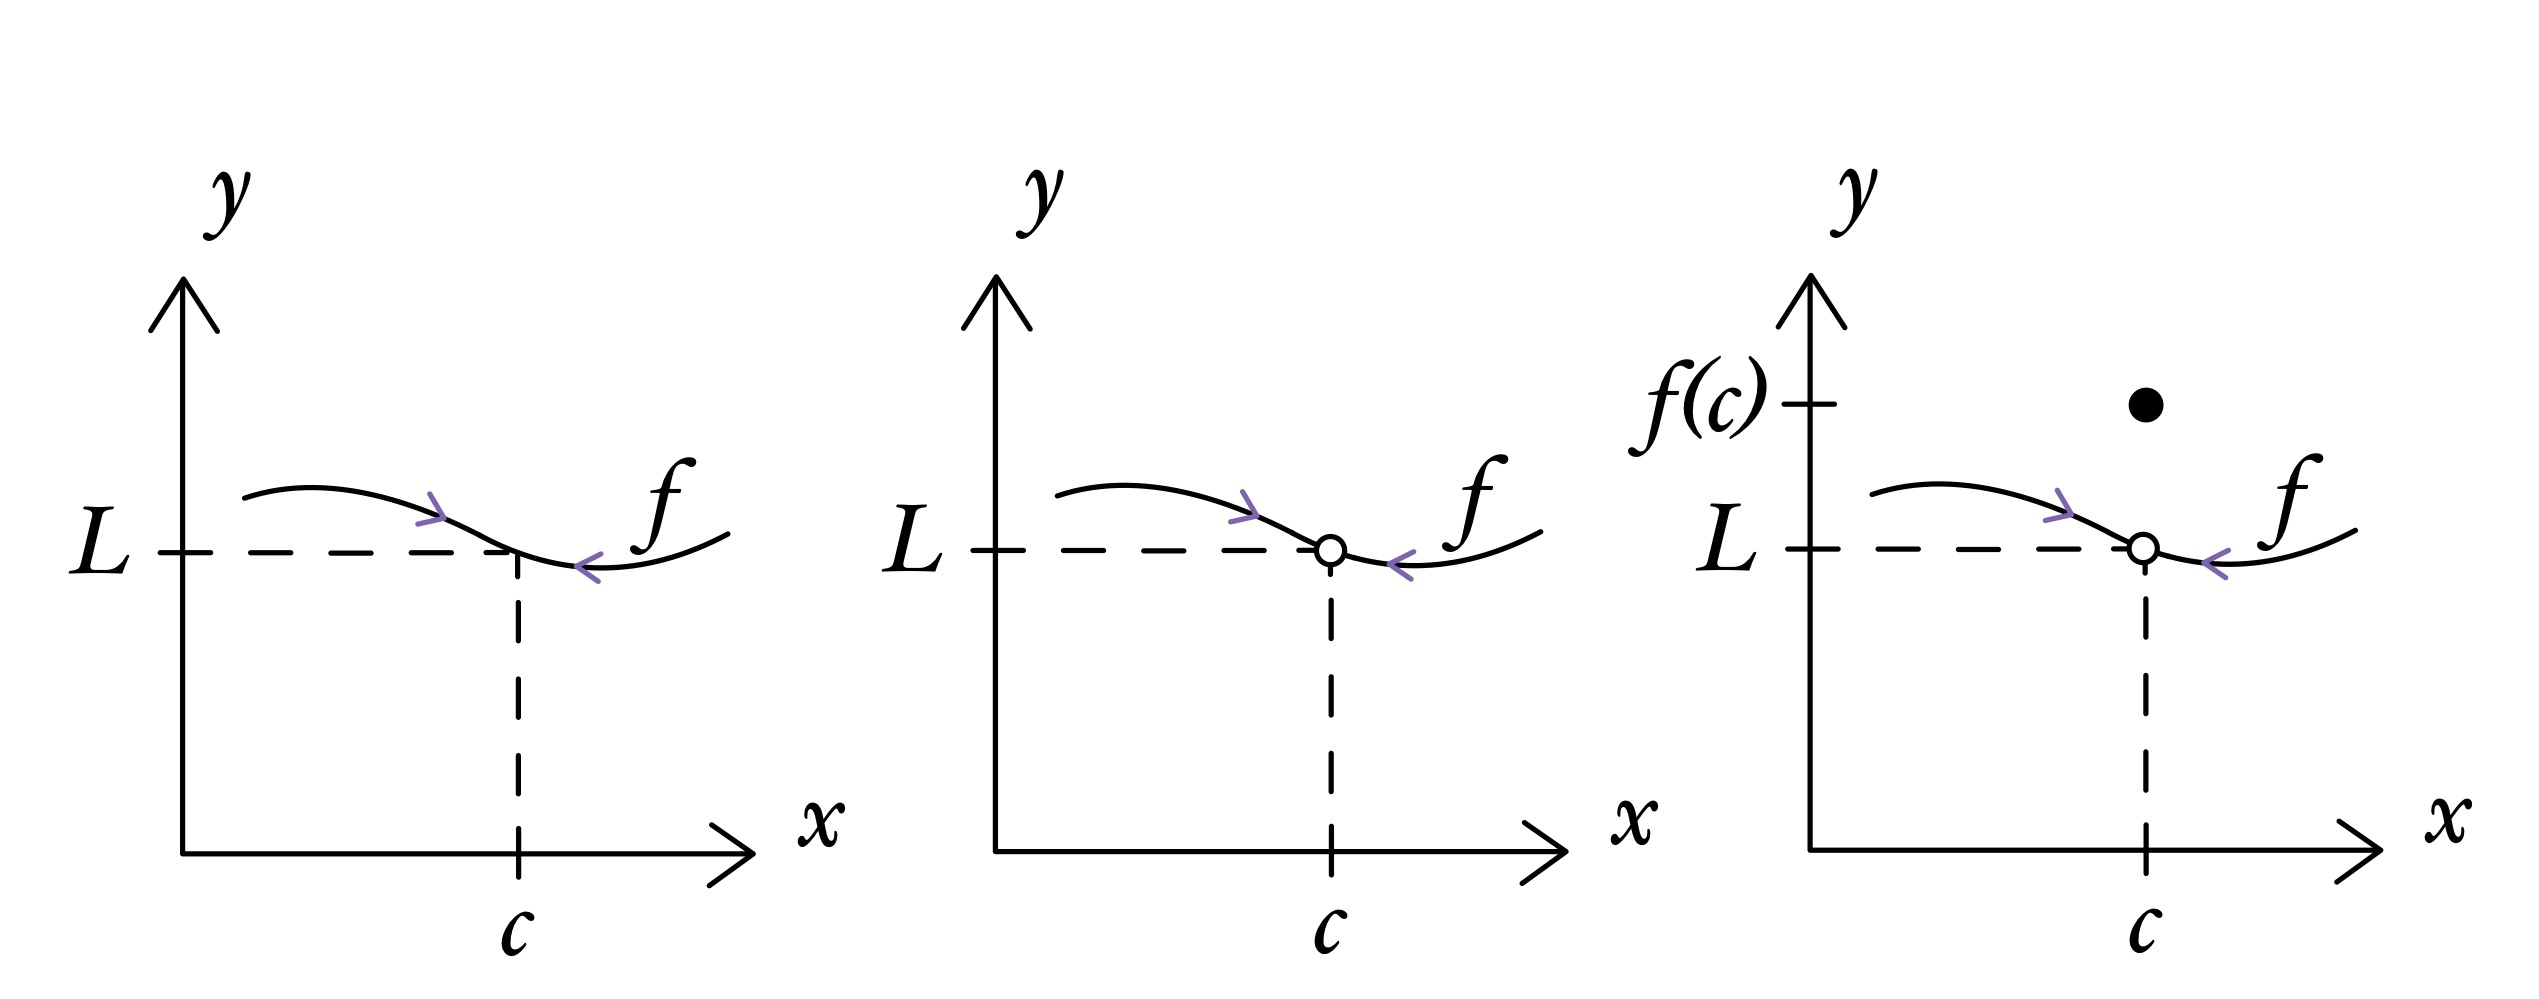
\includegraphics[width=0.7\textwidth]{limit_intuitive.JPG}\figtag{2.1.1}
\end{center}

The first case is that $f(c)=L$. The second case is that $f$ is not defined at $x=c$. The third case is that $f(c)\ne L$. However, in these three cases, $$\lim_{x\to c}f(x)=L.$$

\begin{example}
    Find $\displaystyle\lim_{x\to c_i}f_i(x)$ for the following.
    \begin{enumerate}
        \item $f_1(x)=\dfrac{x^2-9}{x-3}, \quad c_1=3$.
        \item $f_2(x)=\dfrac{x^3-8}{x-2}, \quad c_2=2$.
    \end{enumerate}
\end{example}
\textbf{Solution}. For $\displaystyle\lim_{x\to c_1}f_1(x)$, the function $f_1$ is not defined at $x=3$. However, to find the limit at $x=3$, it does not matter whether $f_1$ is defined at $x=3$ or not. We just care about $f_1$ near $x=3$ but not equal to $3$. For $x\ne 3$, $\dfrac{x^2-9}{x-3}=x+3$. Hence, $\displaystyle\lim_{x\to 3}\dfrac{x^2-9}{x-3}=\lim_{x\to 3}x+3=6$. For $\displaystyle\lim_{x\to c_2}f_2(x)$, the function $f_2$ is not defined at $x=2$. However, for $x\ne 2$, $\dfrac{x^3-8}{x-2}=x^2+2x+4$. Hence, $\displaystyle\lim_{x\to 2}\dfrac{x^3-8}{x-2}=\lim_{x\to 2}x^2+2x+4=12$. \qed

One can make $x$ approach $c$ either from the right side or from the left side. Sometimes, a function cannot have a limit with approaches from both sides. The ``one-sided limits'' may exist. We write $$\lim_{x\to c^-}f(x)=L$$ to indicate that $f(x)$ approaches $L$ when $x$ approaches $c$ from the left, and we write $$\lim_{x\to c^+}f(x)=L$$ to indicate that $f(x)$ approaches $L$ when $x$ approaches $c$ from the right.

\begin{example}
    Find the left-hand-side limit $\displaystyle\lim_{x\to 3^-}f(x)$ and the right-hand-side limit $\displaystyle\lim_{x\to 3^+}f(x)$ in Figure 2.1.2. Note that $f$ is not defined at $x=3$.
\end{example}
\textbf{Solution}. From the figure, we have $\displaystyle\lim_{x\to 3^-}f(x)=2$ and $\displaystyle\lim_{x\to 3^+}f(x)=4$. \qed

\begin{center}
    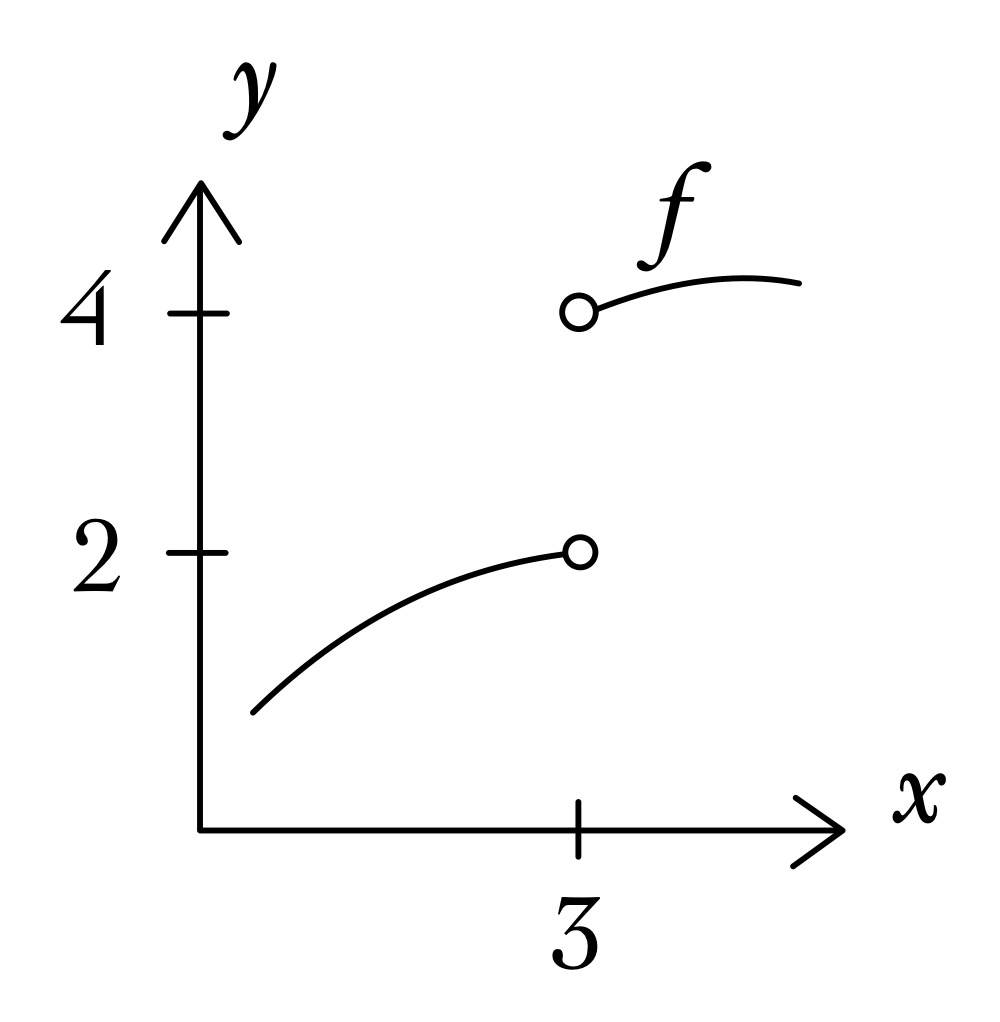
\includegraphics[width=0.7\textwidth/3]{two-side_limits.JPG}\figtag{2.1.2}
\end{center}

For a limit to exist, both the left-hand-side limit and the right-hand-side limit must exist and equal.

\begin{example}
    Let $f(x)=\dfrac{x}{|x|}$ defined on $(-\infty, 0)\cup(0, \infty)$. Note that $f(x)=1$ for $x>0$ and $f(x)=-1$ for $x<0$. Find the two one-sided limits of $f$ at $x=0$ and show that the limit of $f$ at $x=0$ does not exist.
\end{example}
\textbf{Solution}. Since $f(x)=1$ for $x>0$, we easily have $\displaystyle\lim_{x\to 0^+}f(x)=1$ regardless of the fact that $f$ is not defined at $x=0$. Similarly, $\displaystyle\lim_{x\to 0^-}f(x)=-1$. Since the left-hand-side limit and the right-hand-side limit are not equal, the limit does not exist. \qed

\begin{remark}
    For a limit to exist, it must be finite. Otherwise, we say the limit does not exist. However, if a limit does not exist, it might be either oscillating or unbounded (infinite).
\end{remark}

\begin{example}
    In Figure 2.1.3, the limits $\displaystyle\lim_{x\to 3} f(x)$ and $\displaystyle\lim_{x\to 9} f(x)$ do not exist since the function is unbounded near $3$ and $9$.
\end{example}

\begin{center}
    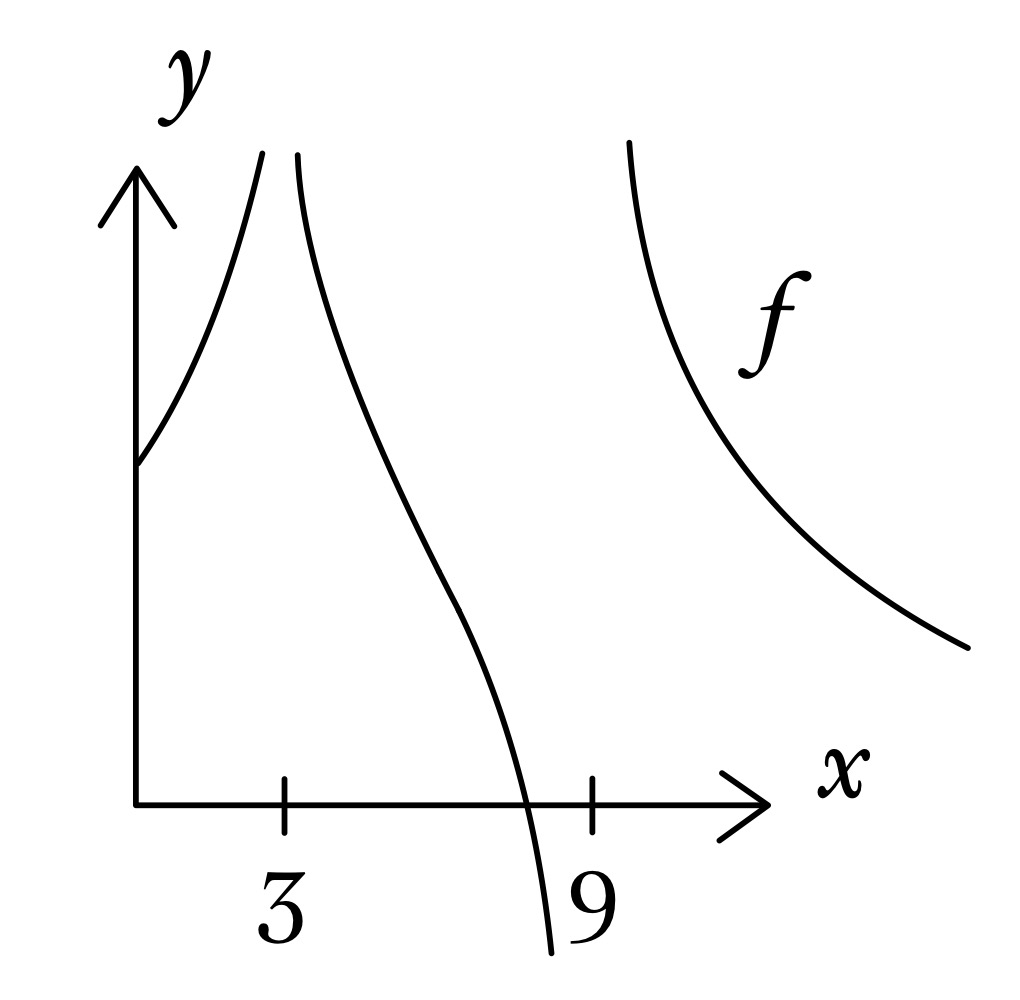
\includegraphics[width=0.26\textwidth]{unbounded_limits.JPG}\figtag{2.1.3}
\end{center}

\begin{example}
    In Figure 2.1.4, the graph of $f(x)=\dfrac{1}{x-2}$ is depicked. As $x$ approaches $4$, $\dfrac{1}{x-2}$ approaches $\dfrac{1}{2}$. Hence, $\displaystyle\lim_{x\to 4}\dfrac{1}{x-2}=\dfrac{1}{2}$. However, as approaches $2$, $\dfrac{1}{x-2}$ gets larger and lager, and $\dfrac{1}{x-2}$ is hence unbounded.
\end{example}

\begin{center}
    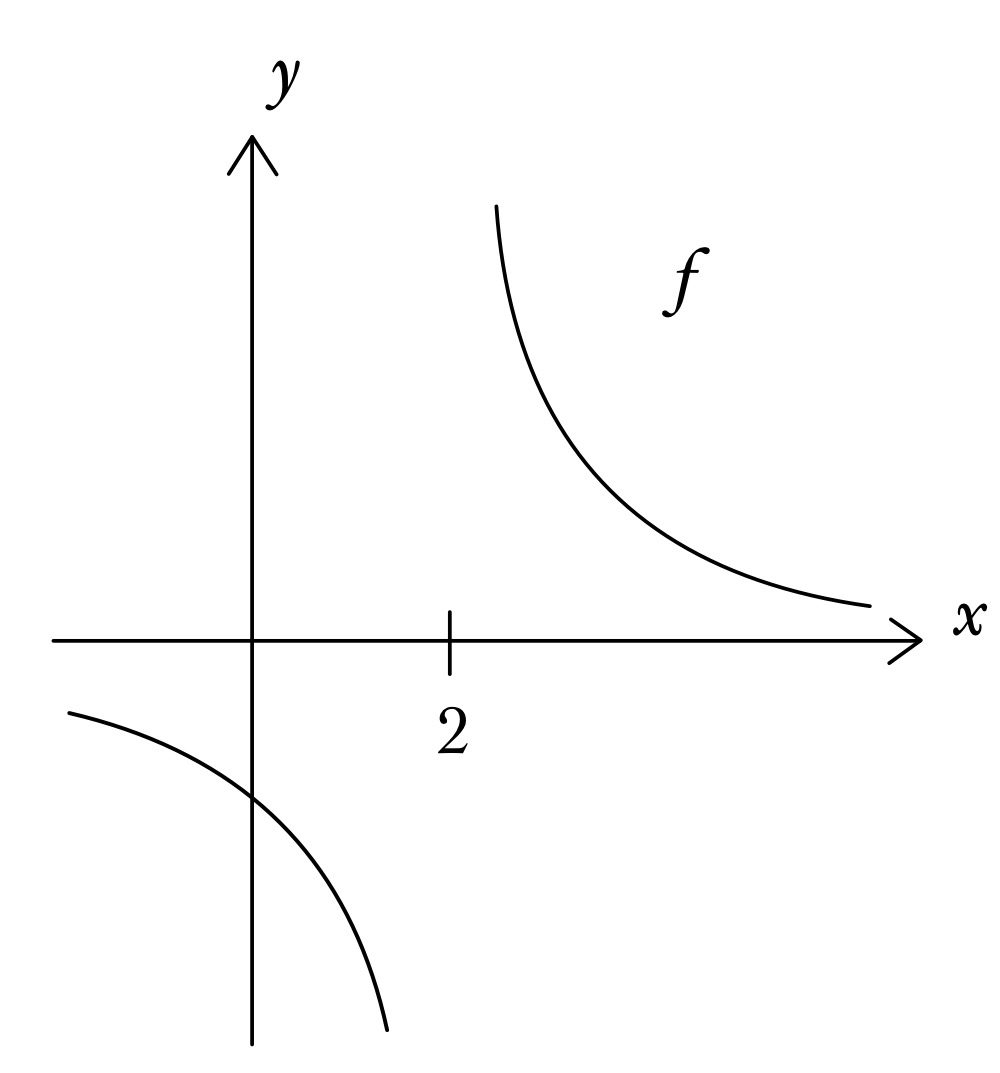
\includegraphics[width=0.34\textwidth]{limit_reciprocal.JPG}\figtag{2.1.4}
\end{center}

\begin{example}
    Let $$f(x)=\left\{\begin{array}{rl}
        1-x^2, \quad & \text{if $x<1$},\\\dfrac{1}{x-1}, \quad & \text{if $x>1$}.
    \end{array}\right.$$ Find the two one-sided limits of $f$ at $x=1$ and show that the limit of $f$ at $x=1$ does not exist.
\end{example}
\textbf{Solution}. For $x<1$, $f(x)=1-x^2$. Thus, $$\lim_{x\to1^-}f(x)=0.$$ For $x>1$, $f(x)=\dfrac{1}{x-1}$. Thus, as $x$ approaches $1$ from the right side, $f(x)$ get larger and larger, and $\dfrac{1}{x-1}$ is hence unbounded. Therefore, $\displaystyle\lim_{x\to 1}f(x)$ does not exist.

\subsection*{Exercise}

\begin{enumerate}[label=\arabic*.]
    \item Find $\displaystyle\lim_{x\to c^-}f(x), \lim_{x\to c^+}f(x), \lim_{x\to c}f(x), f(c)$ with the given graph of $f$ and number $c$.
    \begin{enumerate}
        \item $c=2$.
        \item $c=3$.
        \item $c=3$.
        \item $c=4$.
        \item $c=-2$.
        \item $c=1$.
        \item $c=1$.
        \item $c=-1$.
        \item $c=2$.
        \item $c=3$.
    \end{enumerate}
    \item Decide on intuitive grounds whether the ondicated limit exists. Evaluate it if it exists.
    \begin{enumerate}
        \item $\displaystyle\lim_{x\to 2}2x-1$.
        \item $\displaystyle\lim_{x\to-2}x^2-2x+4$.
        \item $\displaystyle\lim_{x\to 1}2-5x$.
        \item $\displaystyle\lim_{x\to 0}\dfrac{1}{|x|}$.
        \item $\displaystyle\lim_{x\to 3}\dfrac{2x-6}{x-3}$.
        \item $\displaystyle\lim_{x\to 1}x+\dfrac{1}{x}$.
        \item $\displaystyle\lim_{x\to 1}\dfrac{x^2-1}{x-1}$.
        \item $\displaystyle\lim_{x\to 1}\dfrac{x^3-1}{x-1}$.
        \item $\displaystyle\lim_{x\to 1}\dfrac{x^3-1}{x+1}$.
        \item $\displaystyle\lim_{x\to 1}\dfrac{x^2+1}{x^2-1}$.
        \item $\displaystyle\lim_{x\to 0}f(x)$ with $f(x)=\left\{\begin{array}{rl}
            1, \quad & \text{if $x\ne0$},\\
            3, \quad & \text{if $x=0$}.
        \end{array}\right.$
        \item $\displaystyle\lim_{x\to 1}f(x)$ with $f(x)=\left\{\begin{array}{rl}
            3x, \quad & \text{if $x<1$},\\
            3, \quad & \text{if $x>1$}.
        \end{array}\right.$
        \item $\displaystyle\lim_{x\to 4}f(x)$ with $f(x)=\left\{\begin{array}{rl}
            x^2, \quad & \text{if $x\ne4$},\\
            0, \quad & \text{if $x=4$}.
        \end{array}\right.$
        \item $\displaystyle\lim_{x\to 0}f(x)$ with $f(x)=\left\{\begin{array}{rl}
            -x^2, \quad & \text{if $x<0$},\\
            x^2, \quad & \text{if $x>0$}.
        \end{array}\right.$
        \item $\displaystyle\lim_{x\to 0}f(x)$ with $f(x)=\left\{\begin{array}{rl}
            x^2, \quad & \text{if $x<0$},\\
            1+x, \quad & \text{if $x>0$}.
        \end{array}\right.$
        \item $\displaystyle\lim_{x\to 1}f(x)$ with $f(x)=\left\{\begin{array}{rl}
            2x, \quad & \text{if $x<1$},\\
            x^2+1, \quad & \text{if $x>1$}.
        \end{array}\right.$
        \item $\displaystyle\lim_{x\to 0}f(x)$ with $f(x)=\left\{\begin{array}{rl}
            1, \quad & \text{if $x\in\mathbb{Q}$},\\
            -1, \quad & \text{if $x\notin\mathbb{Q}$}.
        \end{array}\right.$
        \item $\displaystyle\lim_{x\to 1}f(x)$ with $f(x)=\left\{\begin{array}{rl}
            2x, \quad & \text{if $x\in\mathbb{Q}$},\\
            2, \quad & \text{if $x\notin\mathbb{Q}$}.
        \end{array}\right.$
    \end{enumerate}
\end{enumerate}

\section{Definition of Limit}



\section{Limit Theorems}



\section{Continuity}





% Formulae for derivatives
\chapter{Derivative and Differentiation}



% Graph drawing, l'Hospital
\chapter{Application of Differentiation}



% Formulae for antiderivatives
\chapter{Integral and Integration}



% sub, IBP
\chapter{Techniques of Integration}



\chapter{Numerical Sequences, Numerical Series, and Power Series}



\chapter{Multivariable Differentiation}



\chapter{Multiple Integrals}


\end{document}